\documentclass[a4paper,11pt,twoside]{memoir}
\setcounter{secnumdepth}{2}
\let\STARTCODE\relax 
\let\STOPCODE\relax 
\STARTCODE
\usepackage{color,calc,graphicx,soul}
\definecolor{nicered}{rgb}{.647,.129,.149} \makeatletter
\newlength\dlf@normtxtw \setlength\dlf@normtxtw{\textwidth}
\def\myhelvetfont{\def\sfdefault{mdput}} \newsavebox{\feline@chapter}
\newcommand\feline@chapter@marker[1][4cm]{
  \sbox\feline@chapter{
    \resizebox{!}{#1}{\fboxsep=1pt
      \colorbox{nicered}{\color{white}\bfseries\sffamily\thechapter}
    }}
  \rotatebox{90}{
    \resizebox{
      \heightof{\usebox{\feline@chapter}}+\depthof{\usebox{\feline@chapter}}}
    {!}{\scshape\so\@chapapp}}\quad
  \raisebox{\depthof{\usebox{\feline@chapter}}}{\usebox{\feline@chapter}}
} \newcommand\feline@chm[1][4cm]{
  \sbox\feline@chapter{\feline@chapter@marker[#1]}
  \makebox[0pt][l]{
    \makebox[1cm][r]{\usebox\feline@chapter}
  }} \makechapterstyle{daleif1}{
  \setlength{\afterchapskip}{10pt}
  \renewcommand{\insertchapterspace}{}
  \renewcommand\chapnamefont{\normalfont\Large\scshape\raggedleft\so}
  \renewcommand\chaptitlefont{\normalfont\huge\bfseries\scshape\color{nicered}}
  \renewcommand\chapternamenum{} 
  \renewcommand\printchaptername{}
  \renewcommand\printchapternum{\vspace{-1.8cm}\null\hfill\feline@chm[2.5cm]\par}
  \renewcommand\afterchapternum{\par\vskip\midchapskip}
  \renewcommand\printchaptertitle[1]{\chaptitlefont\raggedleft
  	##1\par}
  \renewcommand\printchapternonum{\vspace{0.2cm}}
}

\makeatother
\chapterstyle{daleif1}
\STOPCODE
\usepackage[utf8x]{inputenc}
\usepackage[T1]{fontenc}
\usepackage[english, french]{babel}
\usepackage{lipsum}
\usepackage{lmodern}
\rmfamily
\DeclareFontShape{T1}{lmr}{b}{sc}{<->ssub*cmr/bx/sc}{}
\DeclareFontShape{T1}{lmr}{bx}{sc}{<->ssub*cmr/bx/sc}{}
\usepackage{epigraph}
\usepackage[french]{minitoc}
\setcounter{minitocdepth}{2}
\usepackage{soul}
\usepackage[pagebackref,colorlinks=true,citecolor=forestgreen,linkcolor=black,menucolor=alezan,urlcolor=prune]{hyperref}
\renewcommand*{\backref}[1]{}
\renewcommand*{\backrefalt}[4]{
\ifcase #1
-- Non cité.
\or
-- Cité page~#2.
\else
-- Cité pages~#2.
\fi}
\renewcommand*{\backrefsep}{, }
\renewcommand*{\backreftwosep}{ et~}
\renewcommand*{\backreflastsep}{ et~}
\usepackage{lingmacros}
\usepackage{fancybox}
\usepackage{pifont}
\usepackage{dsfont}
\def\sep{\begin{center}\begin{large}\ding{167}\end{large}\end{center}}
\renewcommand{\bibname}{Bibliographie}
\addto{\captionsenglish}{\renewcommand{\bibname}{Bibliographie}}
\addto{\captionsfrench}{\renewcommand{\listfigurename}{Liste des figures}}
\usepackage{newcent}
\usepackage{helvet}
\usepackage{color}
\usepackage{colortbl}
\usepackage{multirow}
\usepackage{longtable}
\newcommand{\withnofdp}[1]{{\NoAutoSpaceBeforeFDP #1}}
\usepackage{arydshln}
\usepackage{listings}
\lstset{
  language=XML, 
  basicstyle=\small,
  showspaces=false,
  showstringspaces=false,
  breaklines=true,
  breakatwhitespace=true,
  morecomment=[s]{<!--}{-->},
  alsoletter=.-,
  commentstyle=\itshape\color{gray},
  markfirstintag=true,
  string=[d]",
  keywords={correction},
  keywordstyle=\color{alizarine},
  stringstyle=\color{acier},
}
\usepackage{pgf,pgfarrows,pgfnodes}
\usepackage{tikz}
\usepackage{tikz-qtree}
\usepackage{tikz-dependency}
\usepackage{pgfplots}
\usetikzlibrary{mindmap,trees, backgrounds}
\usepackage{filecontents}
\usepackage{qtree}
\definecolor{acier}{HTML}{3A8EBA}
\definecolor{alezan}{HTML}{A76726}
\definecolor{alizarine}{HTML}{D90115}
\definecolor{amande}{HTML}{82C46C}
\definecolor{ambre}{HTML}{F0C300}
\definecolor{abricot}{HTML}{E67E30}
\definecolor{grey}{rgb}{0.9,0.9,0.9}
\definecolor{gris}{rgb}{0.1,0.1,0.1}
\definecolor{forestgreen}{rgb}{0.13,0.54,0.13}
\definecolor{dockerblue}{rgb}{0.11,0.56,0.98}
\definecolor{orange}{rgb}{0.64,0.16,0.16}
\definecolor{ocre}{HTML}{DFAF2C}
\definecolor{prune}{HTML}{811453}
\newcommand{\remCyril}[1]{\textcolor{dockerblue}{\emph{CG : #1}}}
\newcommand{\myex}[1]{\color{acier}{\emph{#1}}\color{black}}
\newcommand{\rg}[1]{\textsl{Remarque : #1}}
\def\euro{\mbox{\raisebox{.25ex}{{\it =}}\hspace{-.5em}{\sf C}}}
\newenvironment{changemargin}[2]{\begin{list}{}{
\setlength{\topsep}{0pt}
\setlength{\leftmargin}{0pt}
\setlength{\rightmargin}{0pt}
\setlength{\listparindent}{\parindent}
\setlength{\itemindent}{\parindent}
\setlength{\parsep}{0pt plus 1pt}
\addtolength{\leftmargin}{#1}
\addtolength{\rightmargin}{#2}
}\item }{\end{list}}
\usepackage{chngpage}
\usepackage{amssymb,amsmath,amsthm,amscd}
\usepackage{mathrsfs}
\usepackage{subfig}
\usepackage{tabularx}
\usepackage{calc}
\usepackage{graphicx}
\usepackage{hyperref}
\usepackage{makeidx}
\makeindex
\usepackage[french,intoc,refpage]{nomencl}
\renewcommand{\nomname}{Glossaire}
\renewcommand*{\pagedeclaration}[1]{\unskip\dotfill\hyperpage{#1}}
\makenomenclature
\newcommand{\nocontentsline}[3]{}
\newcommand{\tocless}[2]{\bgroup\let\addcontentsline=\nocontentsline#1{#2}\egroup}
%%%%%%%%%%%%%%%%%%%%%%%%%%%%%%%%%%%%%%%%%%%%%%%%%%%%%%%
%% EN-TETES ET PIEDS DE PAGE
\let\footruleskip\undefined
\usepackage{fancyhdr}
\pagestyle{fancy}% pour activer le style de pages personnalisé
\fancyhf{}%remise à zéro des en-tête et pied de page
\setlength{\headheight}{14pt} % pour fixer la hauteur de l'espace réservé à l'en-tête du haut

%%% Pas de numéro de page sur la première page des chapitres
\makeatletter
\let\ps@plain=\ps@empty
\makeatother

%===================== Style 1 =================================================
%En-tête : 
% * dans la boite de droite (R), pour les pages impaires (O)
% * et dans la boite de gauche (L), pour les pages paires (E)
% mettre le numéro de page (\thepage).
\fancyhead[RO,LE]{% 
\thepage
}
\fancyhead[LO]{\scshape \nouppercase{\rightmark}}  %%%Section
\fancyhead[RE]{\scshape \nouppercase{\leftmark}} %%% Chapitre 
\renewcommand{\headrulewidth}{.4pt}
\fancyfoot{}


%================================== Style 2 ====================================

% \fancyfoot[RO,LE]{% Boite de droite (R), pages impaires(O) et Boites de gauche pages paires
% \thepage
% }
% \fancyhead[CO]{\slshape \nouppercase{\rightmark}}  %%%Section
% \fancyhead[CE]{\slshape \nouppercase{\leftmark}} %%% Chapitre 
% \renewcommand{\headrulewidth}{.4pt}

% Remarques generales :
% nouppercase permet l'affichage en minuscules au lieu de majuscules
% slshape permet l'affichage en lettres penchés
% scshape permet l'affichage en petites capitales

% Pour que les pages paires sans texte (par exemple, à la fin d'un chapitre et
% avant un autre), ne contiennent ni en-tête ni pied de page (source :
% http://www.tex.ac.uk/cgi-bin/texfaq2html?label=reallyblank)
\let\origdoublepage\cleardoublepage
\newcommand{\clearemptydoublepage}{%
  \clearpage
  {\pagestyle{empty}\origdoublepage}%
}
\let\cleardoublepage\clearemptydoublepage

% Réglage fin des notes de bas de page
\FrenchFootnotes % pour les notes de bas de page à la française
\AddThinSpaceBeforeFootnotes % pour avoir une espace fine entre le mot et l'appel de note


%%%%%%%%%%%%%%%%%%%%%%%%%%%%%%%%%%%%%%%%%%%%%%%%%%%%%%%
%% CHAPITRE ETOILE
%% avec référence dans la table des matières et les bons en-têtes
%% il sert pour l'introduction, la page de notations.
\newcommand*\chapterstar[1]{%
  \chapter*{#1}%
  \addcontentsline{toc}{chapter}{#1}%
  \markboth{#1}{#1}}


%%%%%%%%%%%%%%%%%%%%%%%%%%%%%%%%%%%%%%%%%%%%%%%%%%%%%%%
% ENVIRONNEMENTS DE THEOREMES
\theoremstyle{plain} % style plain
\newtheorem{theo}{Théorème}[chapter]
\newtheorem{cor}[theo]{Corollaire}
\newtheorem{prop}[theo]{Proposition}
\newtheorem{lem}[theo]{Lemme}
\newtheorem{conj}[theo]{Conjecture}
\newtheorem*{theoetoile}{Théorème} % théorème non numéroté
\newtheorem*{conjetoile}{Conjecture} % conjecture non numérotée

\theoremstyle{definition} % style definition
\newtheorem{defi}[theo]{Définition}
\newtheorem{exemple}[theo]{Exemple}
\newtheorem{question}[theo]{Question}
\newtheorem{remarque}[theo]{Remarque}
\newtheorem{notation}[theo]{Notation}

% Pour renommer ``preuve'' en ``démonstration''
\renewcommand{\proofname}{Démonstration}


%%%%%%%%%%%%%%%%%%%%%%%%%%%%%%%%%%%%%%%%%%%%%%%%%%%%%%%
% ENVIRONNEMENTS DEDICACE ET EPIGRAPHE
\newenvironment{dedicace}{%
  \newpage\thispagestyle{empty}
  \hfill\begin{minipage}{100mm}\begin{flushright}\it}{%
  \end{flushright}\end{minipage}\vfill}

\newenvironment{epigraphe}{%
  \hfill\begin{minipage}{60mm}\begin{flushright}\footnotesize\it}{%
  \end{flushright}\end{minipage}\hspace*{7mm}\vfill}

\newcommand\tab[1][5mm]{\hspace*{#1}}
\parindent=0em
\begin{document}
\sloppy
\dominitoc
% ================================ Page du garde ==============================

\pdfbookmark[0]{Page de garde}{garde}
\thispagestyle{empty}

\begin{center}
  \begin{tabularx}{\textwidth}{m{10.3cm}m{4cm}}
	 
\includegraphics[width = 3.9cm]{z_images/0_logos/0_inalco.png} %% CG : 3.5cm au lieu de 3 cm
	&
        %% TODO: remplacer le logo du LIMSI par celui de la société ou
        %% du laboratoire où vous avez réalisé votre stage (si le
        %% sujet du mémoire de recherche fait suite à votre stage)
	 
\includegraphics[width = 3.9cm]{z_images/0_logos/1_inria.png} %% CG : 3.5cm au lieu de 3 cm
        \\ \hline
  \end{tabularx}
\end{center}

\begin{center}
\vspace{\stretch{1}}
% Permet de créer un espace vertical de longueur variable (\stretch) et de "poids" 1
{\Large \textbf{Institut National des Langues et Civilisations Orientales}}

\vspace{\stretch{1}}

{\normalsize Département Textes, Informatique, Multilinguisme}

\vspace{\stretch{2}}
\hrule
\vspace{\stretch{1}}
%% TODO: indiquez le titre de votre mémoire
{\LARGE \textbf{Titre du mémoire}}
\vspace{\stretch{1}}
\hrule

\vspace{\stretch{2}}

{\Huge \textsc{Master}}

\vspace{\stretch{1}}

{\LARGE \textsc{Traitement Automatique des Langues}}

\vspace{\stretch{1}}

{\normalsize \emph{Parcours~:}}

\vspace{\stretch{0.5}}

%% TODO: indiquez votre parcours
{\normalsize \emph{Ingénierie Multilingue}}

\vspace{\stretch{1}}

{\large par}

\vspace{\stretch{1}}

%% TODO: indiquez vos nom et prénom
\textbf{{\LARGE Martin \textsc{DIGARD}}}

\vspace{\stretch{2}}

{\normalsize \emph{Directeur de mémoire~:}}

\vspace{\stretch{0.5}}

%% TODO: indiquez le nom du/des directeur(s) de mémoire (enseignant
%% INaLCO qui supervise votre travail)
{\normalsize \emph{Damien NOUVEL}}

\vspace{\stretch{2}}

{\normalsize \emph{Encadrant~:}}

\vspace{\stretch{0.5}}

%% TODO: indiquez le nom du/des encadrant(s) de stage si votre mémoire
%% porte sur votre travail de stage
{\normalsize \emph{Florent JACQUEMARD}}

\vspace{\stretch{2}}

{\normalsize Année universitaire 2020-2021}

\end{center}

\cleardoublepage % pour laisser une page blanche au verso de la page de garde

\newpage
\setcounter{tocdepth}{1}
\pdfbookmark[0]{Table des matières}{tablematieres}
\tocless\tableofcontents
\newpage
\listoffigures
\listoftables
\printnomenclature
\newpage
%%%%%%%%%%%%%%%%%%%%%%%%%%%%%%%%%%%%%%%%%%%%%%%%%%%%%%%%%%%%%%%%%%%%%%%%%%%%%%%%%%


\chapter*{Introduction générale}
\adjustmtc
\addstarredchapter{Introduction générale} 
L’écriture musicale offre de nombreuses possibilités pour un rythme donné. Le contexte musical ainsi que la lisibilité d’une partition pour un batteur entraîné conditionnent les choix d’écritures. Reconnaître la métrique principale d’un rythme, la façon de regrouper les notes par les ligatures, ou simplement décider d’un usage pour une durée parmi les différentes continuations possibles (notes pointées, liaisons, silences, etc.) constituent autant de possibilités que de difficultés.\\Ce mémoire de recherche, effectué en parallèle d’un stage à l’Inria dans le cadre du master de traitement automatique des langues de l’Inalco, contient une proposition d’amélioration de Qparse, un outil de transcription et d’écriture automatique de la musique sur sa capacité à transcrire la batterie. Nous ne parlerons donc pas directement de langues naturelles, mais de l’écriture automatique de partitions de musique à partir de données audios. Cette exercice nécessitera la manipulation d’un langage musical codifié avec une grammaire (solfège, durées, nuances, volumes) et soulèvera des problématiques concernées par les techniques du traitement automatique des langues (TAL).\\
Nous proposons de rechercher des rythmes génériques (\textit{motifs}) en amont dans la chaîne de traitement. Les \textit{motifs} sont prédéfinis avec des combinaisons possibles (\textit{gammes}) qui leur sont associées. Ces \textit{motifs} et leur \textit{gammes} respectives sont appelés \textit{systèmes}. L’usage des \textit{systèmes} a pour objectif de fixer des choix le plus tôt possible dans la chaîne de traitement afin de simplifier le reste des calculs en éliminant une partie d’entre eux. Ces choix concernent notamment la métrique, la séparation des voix ainsi que les règles de réécriture.\\
Nous dresserons dans une première partie, un état de l’art et nous définirons de manière générale le processus de transcription automatique de la musique pour enfin étayer les méthodes utilisées pour la présente proposition. Dans une seconde partie, Le corpus sera présenté ainsi que les différentes expérimentations menées. Nous concluerons par une discussion sur les résultats obtenus et les pistes d’améliorations futures à explorer.


\chapter{Contexte}
\label{chap:05_contexte}
\adjustmtc
\minitoc
\section*{Introduction}
La transcription automatique de la musique (AMT) est un défi ancien \cite{first_one} et difficile qui n’est toujours pas résolu. Il a engendré une pluie de sous-tâches qui ont donné naissance au domaine de la recherche d’information musicale (MIR). Actuellement, de nombreux travaux de MIR font appel au traitement automatique des langues (TAL) \footnote{NLP4MuSA, the 2nd Workshop on Natural Language Processing for Music and Spoken Audio, co-located with ISMIR 2021.}.\\
Dans ce chapitre, nous parlerons de l’informatique musicale, nous tenterons d’établir les liens existants entre le MIR et le TAL ainsi qu’entre les notions de langage musical et langue naturelle. Nous traiterons également de l’utilité et du problème de l’AMT et de la transcription automatique de la batterie (ADT).\\
Enfin, nous décrirons les représentations de la musique qui sont nécessaires à la compréhension du présent travail.
\section{TAL et MIR}
L'informatique musicale\footnote{\url{https://en.wikipedia.org/wiki/Music_informatics}} est une étude du traitement de la musique \cite{book_muller}, en particulier des représentations musicales, de la transformée de Fourier pour la musique\footnote{\url{https://interstices.info/de-fourier-a-la-reconnaissance-musicale/}}, de l'analyse de la structure de la musique et de la reconnaissance des accords. D'autres sujets de recherche en informatique musicale comprennent la modélisation informatique de la musique, l'analyse informatique de la musique, la reconnaissance optique de la musique, les éditeurs audio numériques, les moteurs de recherche de musique en ligne, la recherche d'informations musicales et les questions cognitives dans la musique.\\
Le MIR\footnote{https://ismir.net/}\footnote{https://ismir2021.ismir.net/} apparaît vers le début des années 2000 \cite{MIR_1}. C’est une science interdisciplinaire qui fait appel à de nombreux domaines comme la musicologie, l’analyse musicale, la psychologie, les sciences de l’information, le traitement du
signal que les méthodes d’apprentissage automatisé en informatique et qui a pour but de les catégoriser. Cette discipline récente a notamment été soutenu par de grandes compagnies du web qui veulent développer des systèmes de recommandation de musique ou des moteurs de recherche dédiés au son et à la musique.\\\\
\begin{figure}[!h]
	\centering
	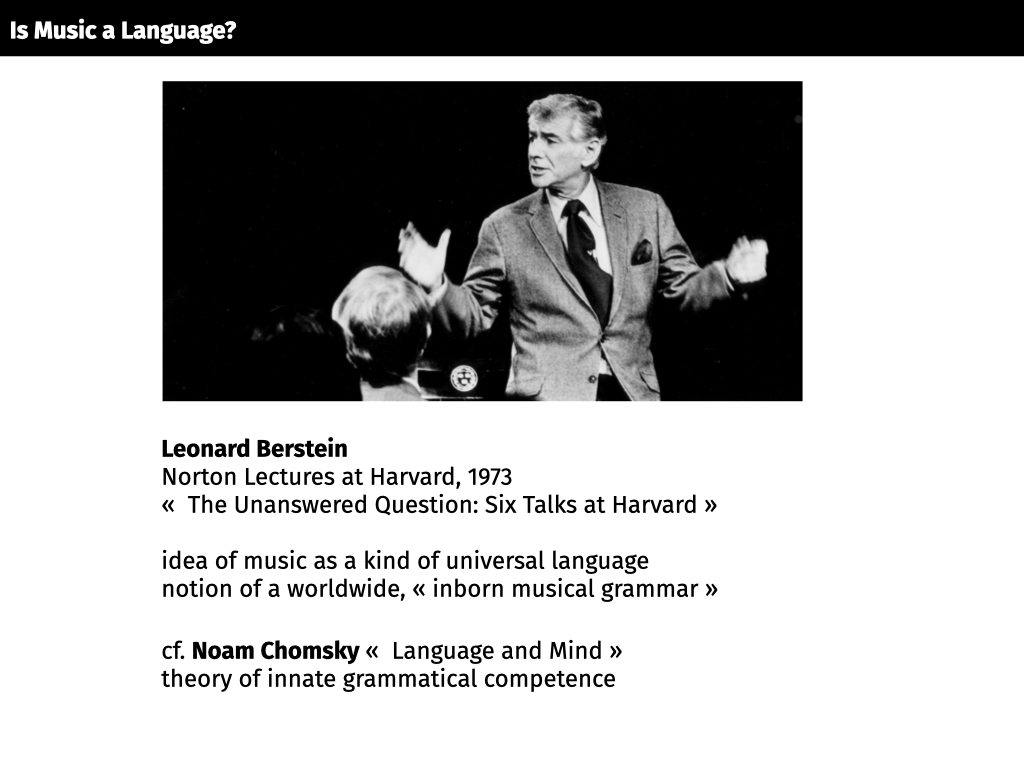
\includegraphics[height=85mm, width=125mm]{z_images/1_automatic_transcription/Bernstein.png}
\end{figure}\\
Aborder la musique à travers le TAL nécessite une réflexion autour de la musique en tant que langage ainsi que la possibilité de comparer ce même langage avec les langues naturelles. Quelques travaux en neuroscience ont abordé la question, notamment par observation des processus cognitifs et neuronaux que les systèmes de traitement de ces deux langages avaient en communs. Dans le travail de Poulin-Charronnat et al. \cite{poulincharronnat:hal-01985213}, la musique est reconnue comme étant un système complexe spécifique à l’être humain dont une des similitudes avec les langues naturelles est l’émergence de régularités reconnues implicitement par le système cognitif. La question de la pertinence de l’analogie entre langues naturelles et langage musical a également été soulevée à l’occasion de projets de recherche en TAL. Keller et al. \cite{keller:hal-03279850} ont exploré le potentiel de ces techniques à travers les plongements de mots et le mécanisme d’attention pour la modélisation de données musicales. La question du sens d’une phrase musicale apparaît, selon eux, à la fois comme une limite et un défi majeur pour l’étude de cette analogie.\\\\
\textit{Ici, Digression sur la musicologie calculatoire vs linguistique computationnelle ?}\\\\
D’autres travaux très récents, ont aussi été révélés lors de la \textit{première conférence sur le NLP pour la musique et l'audio (NLP4MusA 2020)}. Lors de cette conférence, Jiang et al. \cite{Jiang2020DiscoveringMR} ont présenté leur implémentation d’un modèle de langage musical auto-attentif visant à améliorer le mécanisme d'attention par élément, déjà très largement utilisé dans les modèles de séquence modernes pour le texte et la musique.\\
Il semblerait que le domaine du TAL qui se rapproche le plus du MIR serait la reconnaissance de la parole. En effet, la séparation des sources ont des approches similaires dans les deux domaines. De plus, il y a un lien entre partition musicale comme manière d’écrire la musique et texte comme manière d’écrire la parole.\\
Similitudes :\\
Reconnaissance automatique de la parole :\\
signal $\Rightarrow$ phonèmes $\Rightarrow$ texte
Transcription automatique de la musique :\\
signal $\Rightarrow$ MIDI $\Rightarrow$ partition
Différence :\\
Texte (données linéaires) ≠ partition (données structurées hiérarchiques)
\section{La transcription automatique de la musique}
%\subsection{Transcription musicale}
En musique, la transcription\footnote{\url{https://en.wikipedia.org/wiki/Transcription_(music)}} est la pratique consistant à noter un morceau ou un son qui n'était auparavant pas noté et/ou pas populaire en tant que musique écrite, par exemple, une improvisation de jazz ou une bande sonore de jeu vidéo. Lorsqu'un musicien est chargé de créer une partition à partir d'un enregistrement et qu'il écrit les notes qui composent le morceau en notation musicale, on dit qu'il a créé une transcription musicale de cet enregistrement.\\
%\subsection{Automatisation}
L'objectif de la transcription automatique de la musique (AMT) \cite{article1} est de convertir la performance d'un musicien en notation musicale - un peu comme la conversion de la parole en texte dans le traitement du langage naturel. L’AMT a des intérêt multiples, notemment pour la transcription de solos ou encore pour la constitution de corpus musicologiques. Ces deux aspects sont valables dans n’importe quels domaines musicaux dans lequels les partitions seraient inexistantes. Par exemple, dans les domaines oraux ou d’improvisation qui manquent de partition (jazz, pop) \cite{article1}.\\
Comme déjà évoqué précédemment, il s’agit d’un problème ancien et difficile. C’est un « graal » de l’informatique musicale. En 1976, H. C. Longuet-Higgins \cite{first_one} évoquait déjà la représentation musicale en arbre syntaxique dans le but d’écrire automatiquement des partitions à partir de données audio en se basant sur un mimétisme psychologique de l’approche humaine. De même pour les chercheurs en audio James A. Moorer, Martin Piszczalski et Bernard Galler qui, en 1977\footnote{\url{https://en.wikipedia.org/wiki/Transcription_(music)}}, ont utilisé leurs connaissances en ingénierie de l’audio et du numérique pour programmer un ordinateur afin de lui faire analyser un enregistrement musical numérique de manière à détecter les lignes mélodiques, les accords et les accents rythmiques des instruments à percussion.\\
%\subsection{Le processus général}
La tâche de transcription automatique de la musique comprend deux activités distinctes : l'analyse d'un morceau de musique et l'impression d'une partition à partir de cette analyse.\\\\
%\subsection*{Exemple de sous-tâche dans la figure 1.1 remplace ARCHITECTURE}
La figure \ref{AMT_presentation} est une proposition de Benetos et Al. \cite{article1} qui représente l'architecture générale d'un système de transcription musicale. On y observe plusieurs sous-tâches de l’AMT :
\begin{itemize}
	\item La séparation des sources à partir de l’audio.
	\item Le système de transcription :
	\begin{itemize}
		\item Cœur du système :\\
		$\Rightarrow$ Algorithmes de détection des multi-pitchs et de suivi des \tab notes.\\
		Quatres sous-tâches optionnelles accompagnent ces algorithmes :
		\begin{itemize}
			\item identification de l'instrument ;
			\item estimation de la tonalité et de l'accord ;
			\item détection de l'apparition et du décalage ;
			\item estimation du tempo et du rythme.
		\end{itemize}
	\end{itemize}
	\item Apprentissage sur des modèles accoustiques et musicologiques.
	\item \textit{Optionnel :} Informations fournies de manière externe. Soit fournis en amont (genre, instruments,…), soit par interaction avec un utilisateur (infos sur une partition incomplète).
\end{itemize}
\begin{figure}[!h]
	\centering
	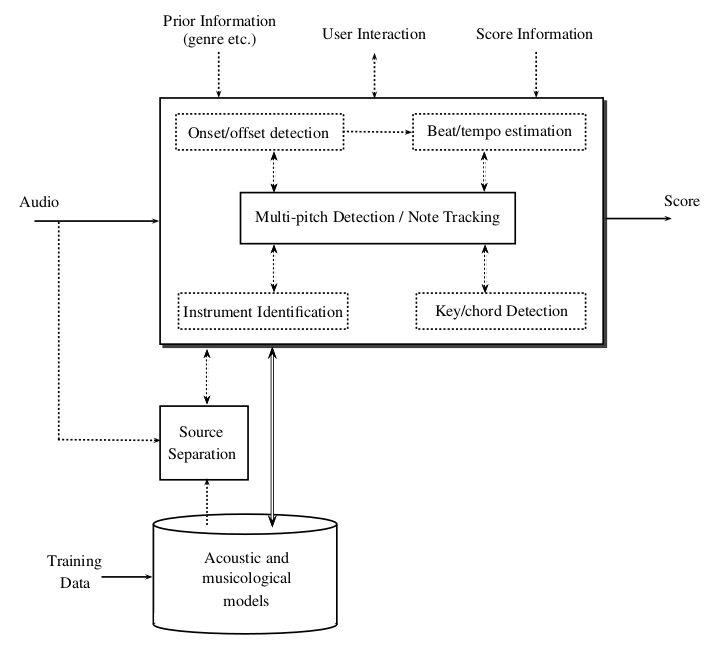
\includegraphics[height=95mm, width=130mm]{z_images/1_automatic_transcription/0_general_process.png}
	\caption{Transcription automatique}
	\label{AMT_presentation}
	\textit{Les sous-systèmes et algorithmes optionnels sont présentés à l'aide de lignes pointillées. Les doubles flèches mettent en évidence les connexions entre les systèmes qui incluent la fusion d'informations et une communication plus interactive entre les systèmes.}
\end{figure}\newpage
\section{La transcription automatique de la batterie}
La batterie est un instrument récent qui s’est longtemps passé de partition. En effet pour un batteur, la qualité de lecteur lorsqu’elle était nécessaire, résidait essentiellement dans sa capacité à lire les partitions des autres instrumentistes (par exemple, les grilles d’accords et la mélodie du thème en jazz) afin d’improviser un accompagnement approprié que personne ne pouvait écrire pour lui à sa place.\\
Les partitions de batterie sont arrivées par nécessité avec la pédagogie et l’émergence d’écoles de batterie partout dans le monde. Un autre facteur qui a contribué à l’expansion des partitions de batterie est l’arrivée de la musique assistée par ordinateur (MAO). En effet, l’usage de boîte à rythmes ou de séquenceurs permettant d’expérimenter soi-même l’écriture de rythmes en les écoutant mixés avec d’autres instruments sur des machines a permis  aux compositeurs de s’émanciper de la création d’un batteur en lui fournissant une partition contenant les parties exactes qu’ils voulaient entendre sur leur musique.\\
%\subsection{Utilité et problème de l’ADT}
La batterie a un statut à part dans l’univers de l’AMT puisqu'il s'agit d'instruments sans hauteur (du point de vue harmonique), d'événements sonores auxquels une durée est rarement attribuée et de notations spécifiques (symboles des têtes de notes).\\
Les applications de l’ADT seraient utiles dans tous les domaines musicaux contenant de la batterie mais aussi de manière plus générale dans le domaine du MIR. Si les ordinateurs étaient capables d'analyser la partie de la batterie dans la musique enregistrée, cela permettrait une variété de tâches de traitement de la musique liées au rythme. En particulier, la détection et la classification des événements sonores de la batterie par des méthodes informatiques est considérée comme un problème de recherche important et stimulant dans le domaine plus large de la recherche d'informations musicales \cite{8350302}.\\
\section{Les représentations de la musique}
\subsection*{Les données audio}
Le fichier WAV\footnote{https://en.wikipedia.org/wiki/WAV} est une instance du Resource Interchange File Format (RIFF) défini par IBM et Microsoft. Le format RIFF agit comme une "enveloppe" pour divers formats de codage audio.
Bien qu'un fichier WAV puisse contenir de l'audio compressé, le format audio WAV le plus courant est l'audio non compressé au format LPCM (linear pulse-code modulation). Le LPCM est également le format de codage audio standard des CD audio, qui stockent des données audio LPCM à deux canaux échantillonnées à 44 100 Hz avec 16 bits par échantillon. Comme le LPCM n'est pas compressé et conserve tous les échantillons d'une piste audio, les utilisateurs professionnels ou les experts en audio peuvent utiliser le format WAV avec l'audio LPCM pour obtenir une qualité audio maximale.
\subsection*{Les données MIDI}
Le MIDI\footnote{\url{https://en.wikipedia.org/wiki/MIDI}} (Musical Instrument Digital Interface) est une norme technique qui décrit un protocole de communication, une interface numérique et des connecteurs électriques permettant de connecter une grande variété d'instruments de musique électroniques, d'ordinateurs et d'appareils audio connexes pour jouer, éditer et enregistrer de la musique.\\\\
Les données midi sont représentées sous forme de piano-roll. Chaque points sur la figure \ref{piano_roll} est appelé « évènement midi » :
\begin{figure}[!h]
	\centering
	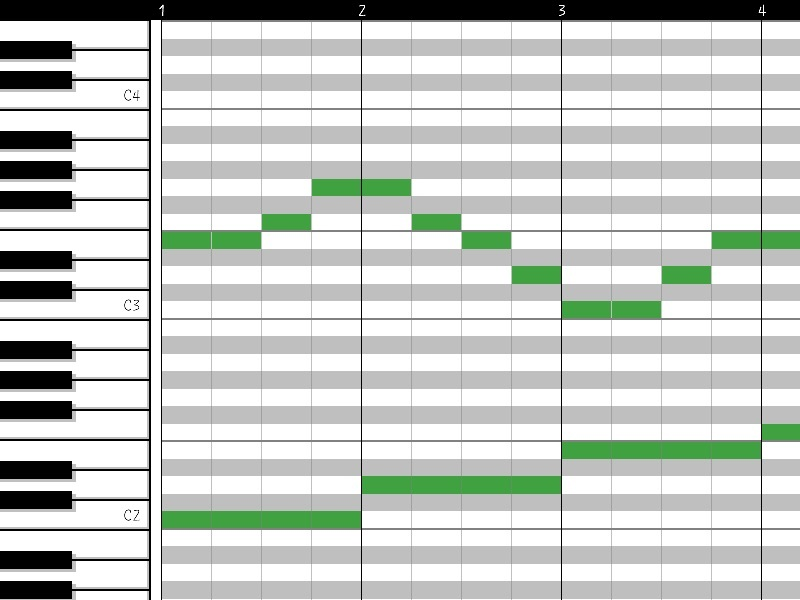
\includegraphics[height=40mm, width=50mm]{z_images/2_midi/exemple_midi_piano.jpg}
	\caption{Exemple évènements avec durée}
	\label{piano_roll}
\end{figure}\\
Chaque évènement MIDI rassemble un ensemble d’informations sur la hauteur, la durée, le volume, etc… :
\begin{figure}[h!]
	\centering
	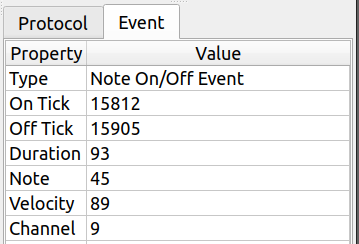
\includegraphics[height=40mm, width=50mm]{z_images/2_midi/representation_numerique_1.png}
	\caption{Critère pour un évènement}
\end{figure}\newpage
Pour la batterie, les évènements sont considérés sans durée, nous ignorerons donc les offsets (« Off Event »), les « Off Tick » et les « Duration ». Le channel ne nous sera pas utile non-plus.\\
\textit{Ici, définir Tick et channel.}\\\\
Voici un exemple de piano-roll midi pour la batterie :
\begin{figure}[h!]
	\centering
	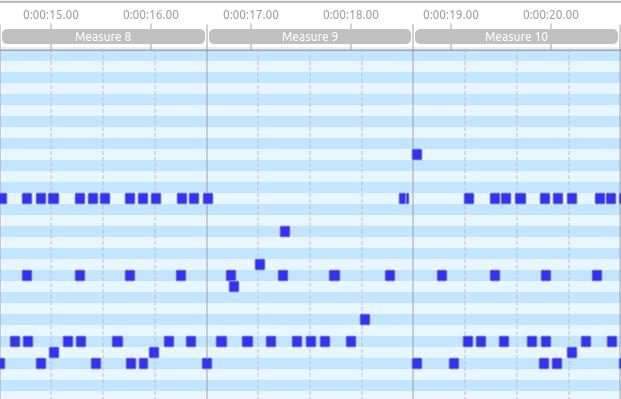
\includegraphics[height=40mm, width=50mm]{z_images/2_midi/representation_numerique_0.png}
	\caption{Exemple évènements sans durée}
\end{figure}\\
On observe que toutes les durées sont identiques.
\subsection*{Les partitions}
\begin{figure}[h!]
	\centering
	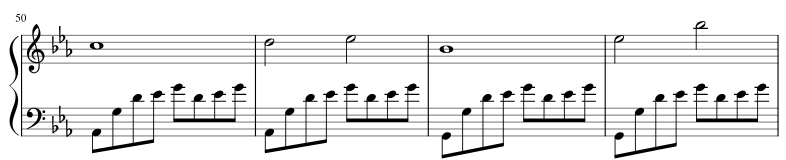
\includegraphics[height=30mm, width=120mm]{z_images/1_automatic_transcription/exemple_partoche.png}
	\caption{Exemple de partition de piano}
\end{figure}
Une partition de musique\footnote{\url{https://fr.wikipedia.org/wiki/Partition\_(musique)}} est un document qui porte la représentation systématique du langage musical sous forme écrite. Cette représentation est appelée transcription et elle sert à traduire les quatre caractéristiques du son musical :
\begin{itemize}
	\item la hauteur ;
	\item la durée ;
	\item l'intensité ;
	\item le timbre.
\end{itemize}
Ainsi que de leurs combinaisons appelées à former l'ossature de l'œuvre musicale dans son déroulement temporel, à la fois :
\begin{itemize}
	\item diachronique (succession des instants, ce qui constitue en musique la mélodie) ;
	\item et synchronique (simultanéité des sons, c'est-à-dire l'harmonie).
\end{itemize}
\section*{Conclusion}
Dans ce chapitre, nous avons établi que le MIR s’intéresse de plus en plus au TAL, et que par ce biais, il y a des liens possibles entre le langage musical et les langues naturelles, le plus proche étant probablement le phénomène d’écriture des sons de l’un comme l’autre.\\
Nous avons également établi que le MIR est né de l’AMT qui est un problème ancien et très difficile et qu’il serait toujours très utile de le résoudre (autant pour l’AMT que pour l’ADT).\\
Et enfin, nous avons décrit les représentations de la musique nécessaires à la compréhension du présent mémoire, allant du son jusqu’à l’écriture.

\chapter{État de l’art}
\label{chap:articles}
\minitoc
\section*{Introduction}
Dans ce chapitre, nous observerons les différentes avancées qui ont déjà eues lieues dans le domaine de la transcription automatique de la musique et de la batterie afin de situé notre démarche.\\
Nous aborderons le passage crucial du monophonique au polyphonique dans la transcription. Nous ferons un point sur les deux grandes parties de l’AMT de bout en bout : de l’audio vers le MIDI puis des données MIDI vers l’écriture d’une partition. Ensuite, nous ferons une critique des approches linéaires et des approches hiérarchiques. Enfin, nous ferons un bilan afin de situer l’ADT dans l’état de l’art de l’AMT.
\section{Monophonique et Polyphonique}
Les premiers travaux ont été faits sur l’identification des instruments monophoniques\footnote{Une seule note à la fois, ou plusieurs notes de même durée (monophonie par accord).}\cite{future_directions}. Actuellement, le problème de l'estimation automatique de la hauteur des signaux monophoniques peut être considéré comme résolu, mais dans la plupart des contextes musicaux, les instruments sont polyphoniques.\\
L'estimation des hauteurs multiples (détection multi-pitchs ou F0 multiples) est le problème central de la création d'un système de transcription de musique polyphonique. Il s’agit de la détection de notes qui peuvent apparaître simultanément et être produites par plusieurs instruments différents. Ce défi est donc majeur pour la batterie puisque c’est un instrument qui est lui-même constitué de plusieurs instruments.\\
Le fort degrés de chevauchement entre les durées ainsi qu’entre les fréquences complique l’identification des instruments polyphoniques. Cette tâche est étroitement liées à la séparation des sources et concerne aussi la séparation des voix. Les performances des systèmes actuels ne sont pas encore suffisantes pour permettre la création d'un système automatisé capable de transcrire de la musique polyphonique sans restrictions sur le degré de polyphonie ou le type d'instrument. Cette question reste donc encore ouverte. 
\section{Audio vers MIDI}
Utilité de l’audio vers MIDI dans la vraie vie $\Rightarrow$ p. 4 et 5 de \cite{Review_ADT}.\\\\
La plupart des travaux se sont concentrés sur le traitement du signal vers la génération du midi \cite{AMT_for_2_Instru}. Cette partie englobe plusieurs sous-tâches dont la détection multi-pitchs, la détection des onset et des offset, l'estimation du tempo, la quantification du rythme, la classification des genres musicaux,…\\
En ADT\cite{Review_ADT}, plusieurs stratégies de répartition Pre/Post-processing sont possibles pour la détection multi-pitchs. Une des démarches intuitives serait de la préparer dès le préprocessing, dans le pré-traitement, pendant la séparation des sources en supprimant les features non-pertinentes pour une meilleure détection des instruments de la batterie. Par exemple, en supprimant la structure harmonique pour atténuer l’influence des instruments à hauteurs sur la détection grosse-caisse et caisse-claire. Mais certaines études montrent que des expériences similaires ont donné des résultats non-concluants et que la suppression des instruments à hauteurs peut avoir des effets néfastes sur les performances de l’ADT. Cependant, les systèmes d’ADT basés sur des RNN ou des NMF font la séparation des sources pendant l’optimisation ce qui réduit la nécessité de la faire pendant le préprocessing.\\
Pour la reconnaissance des instruments, une approche possible\cite{Eronen} est de mettre un modèle probabiliste dans l’étape de la classification des évènements afin de classer les différents sons de la batterie. Dans cette méthode, on se place de sample audio isolés en modélisant la progression temporelle des features avec un HMM. Les features sont transformés en représentations statistiques indépendantes.
L’approche AdaMa\cite{adama_1} est une autre approche de la même catégorie, elle commence par une estimation initiale des sons de la batterie qui sont itérativement raffinés pour matcher l’enregistrement visé.\\
- Extraction of rhythmic information (tempo, beat, and musical timing)\\
\section{MIDI vers partition}
Lorsque les travaux principaux parlent de transcription de bout en bout, l’appellation « score » (\textit{partition}) désigne souvent un ouput au format Music XML, ou simplement MIDI. Par exemple, dans \cite{SHIBATA2021262}, la chaîne de traitement va jusqu’à la génération d’une séquence MIDI quantifiée qui est importée dans MuseScore pour en extraire manuellement un fichier MusicXML contenant plusieurs voix.\\
Seuls quelques travaux récents s’intéressent de près à la création d’outils permettant la génération de partition. Le problème de la conversion d'une séquence d'événements musicaux symboliques en une partition musicale structurée est traité notamment dans \cite{foscarin:hal-01988990}. Ce travail, qui vise à résoudre en une fois la quantification du rythme et la production de partition, s’appuie tout au long du processus sur  des grammaires génératives qui fournissent un modèle hiérarchique à priori des partitions. Les expériences ont des résultats prometteurs, mais il faut relevé qu’elle ont été menées avec un ensemble de données composé d'extraits monophoniques, il reste donc a traiter le passage au polyphonique en couplant le problème de la séparation des voix avec la quantification du rythme.\\
L'approche de \cite{foscarin:hal-01988990} est fondée sur la conviction que la complexité de la structure musicale dépasse les modèles linéaires.
\section{Approche linéaire et approche hiérarchique}
Plusieurs travaux ont d’abord privilégié l’approche stochastique. Par exemple, Shibata et al.\cite{SHIBATA2021262} ont utilisé le modèle de Markov caché (HMM)\footnote{\url{https://fr.wikipedia.org/wiki/Modèle_de_Markov_caché}}\footnote{\url{https://en.wikipedia.org/wiki/Hidden_Markov_model}} pour la reconnaissance de la métrique. Ils utilisent d’abord deux réseaux de neurones profonds, l’un pour la reconnaissance des pitchs et l’autre pour la reconnaissance de la vélocité. Pour la dernière couche, la probabilité est obtenue par une fonction sigmoïde. Ils construisent ensuite plusieurs HMM métriques étendus pour la musique polyphonique correspondant à des métriques possibles et ils calculent la probalitité maximale pour chaque modèle afin d’obtenir la métrique la plus probable.
\begin{figure}[h]
	\centering
	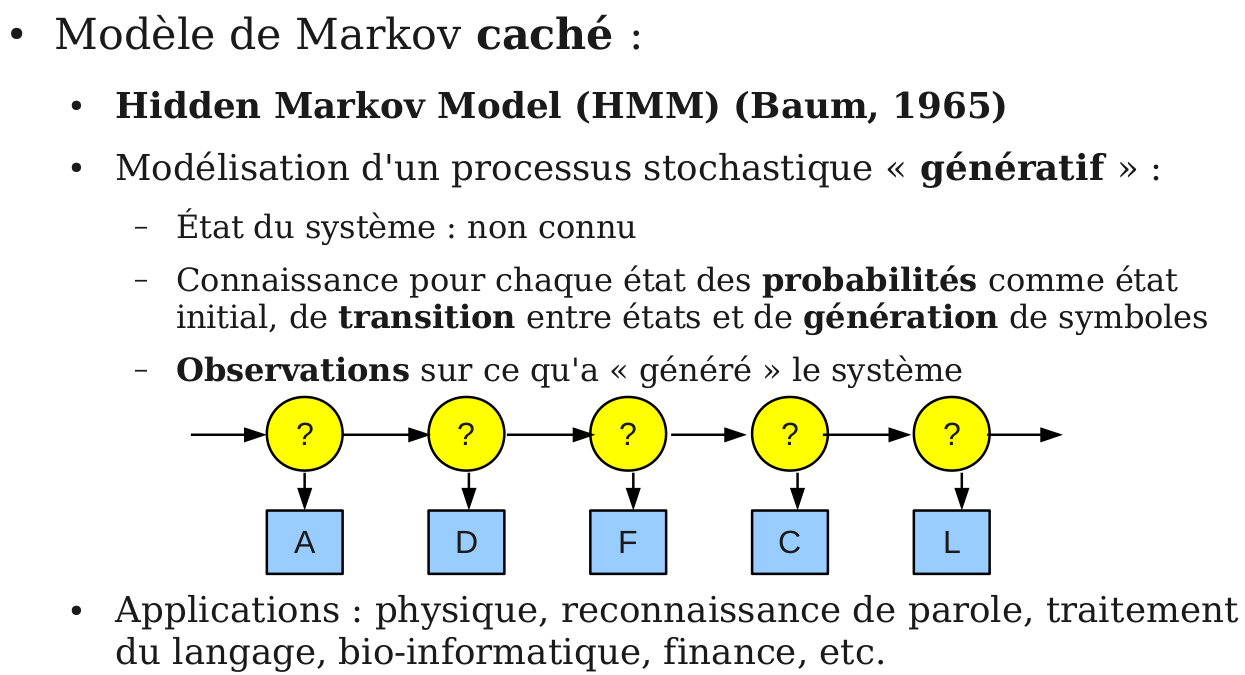
\includegraphics[height=50mm, width=90mm]{z_images/2_etat_de_l_art/hmm.png}
	\caption{HMM}
	\textit{Source : Cours de Damien Nouvel\footnote{\url{https://damien.nouvels.net/fr/enseignement}}}
\end{figure}
L’évaluation finale des résultats de \cite{SHIBATA2021262}, montre qu’il faut rediriger l’attention vers les valeurs des notes, la séparation des voix et d'autres éléments délicats de la partition musicale qui sont significatifs pour l'exécution de la musique. Hors, même si la quantification du rythme se fait le plus souvent par la manipulation de données linéaires allant notamment des real time units (secondes) vers les musical time units (temps, métrique,…), de nombreux travaux suggèrent d’utiliser une approche hiérarchique puisque le langage musical est lui-même structuré. En effet, ces structures (notamment les arbres syntaxiques) sont idéales pour représenter le langage musical.
Une méthodologie simple pour la description et l'affichage des structures musicales est présenté dans \cite{rythm_tree}. Les RT y sont évoqués comme permettant une cohésion complète de la notation musicale traditionnelle avec des notations plus complexes. Jacquemards et al.\cite{jacquemard:hal-01134096} propose aussi une représentation formelle du rythme sous forme d'arbre, inspirée de modèles théoriques antérieurs et dont l’objectif est la réécriture de termes. La réécriture d’arbres, dans un contexte de composition assistée par ordinateur par exemple, pourrait permettre de suggérer à un utilisateur diverses notations possibles pour une valeur rythmique, avec des complexités différentes. La nécessité d’une approche hiérarchique pour la production automatique de partition est évoquée dans \cite{foscarin:hal-01988990}. Les modèles de grammaire qui y sont exposés sont différents de modèles markoviens linéaires de précédent travaux.\newpage
\begin{figure}[h]
	\centering
	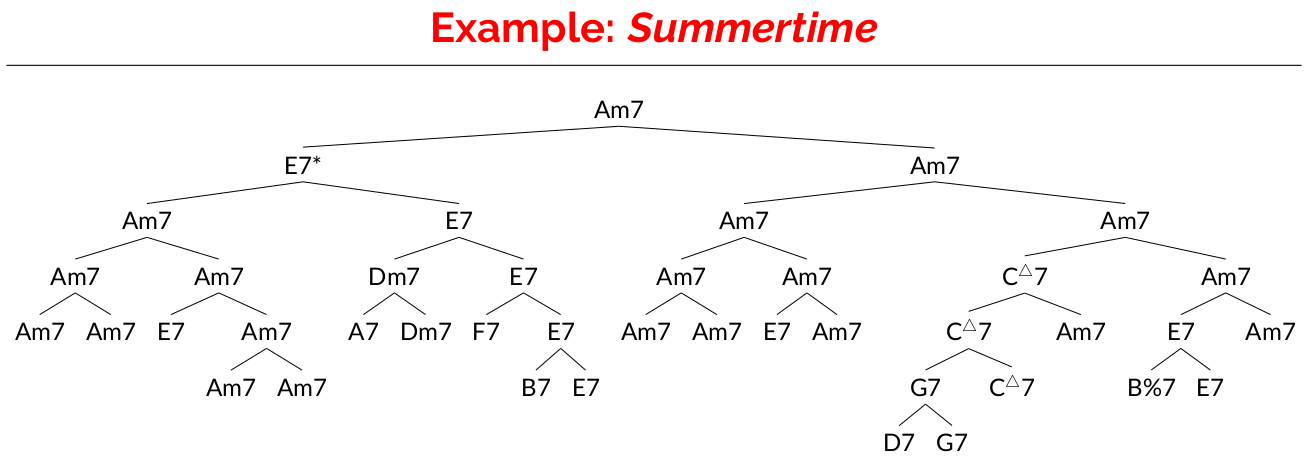
\includegraphics[height=40mm, width=120mm]{z_images/2_etat_de_l_art/summertime_tree.png}
	\caption{arbre\_jazz}
	\textit{Représentation arborescente d’une grille harmonique}\cite{harasimjazz}
\end{figure}
\section*{Conclusion}
\begin{itemize}
	\item Personne fait du MIDI vers partition ;
	\item Pas de formalisation de la notation de la batterie ;
	\item bla bla…
\end{itemize}
Un grand nombre travaux ont déjà été menés dans le domaine de l’ADT. La plupart ont été énumérés par Wu et al. \cite{Review_ADT} qui, pour mieux comprendre la pratique des systèmes d’ADT, se concentrent sur les méthodes basées sur la factorisation matricielle non négative et celles utilisant des réseaux neuronaux récurrents.\\
La plupart des travaux déjà entrepris se concentrent sur des méthodes de calcul pour la détection d'événements sonores de batterie à partir de signaux acoustiques ou sur la séparation entre les évènement sonore de batterie avec ceux des autres instruments dans un orchestre ou un groupe de musique \cite{2802}, ainsi que sur l'extraction de caractéristiques de bas niveau telles que la classe d'instrument et le moment de l'apparition du son. Très peu d'entre eux ont abordé la tâche de générer des partitions de batterie.
Nous avons décidé de compléter le travail qui concerne la batterie en commençant par l’endroit le moins pratiqué, à savoir la transcription du MIDI vers la partition.

\chapter{Méthodes et contributions}
\label{chap:07_methodes_et_contributions}
\minitoc
\section{Introduction}
Dans ce chapitre, nous expliquerons en détails les méthodes que nous avons employées pour l’ADT. Nous commencerons par une description de qparse et des arbres de rythmes. Nous proposerons ensuite une modélisation comprenant une description de la notation de la batterie mise en relation avec les informations MIDI, ceci ayant pour objectif le parsing des données MIDI en arbre syntaxique. Enfin, nous démontrerons un modèle théorique de pattern (implémentable) qui devra être utilisé comme base de connaissance pour obtenir un système plus rapide et une meilleure qualité en sortie.
\section{Les méthodes}
\subsection{Qparse}
%\subsubsection{Qparse}
Qparse produit une partition musicale en prenant en entrée une performance musicale symbolique (par exemple un fichier MIDI) et un automate à arbre pondéré décrivant un langage de rythmes préférés (grammaire pondérée). La quantification des rythmes est basée sur des algorithmes d’analyse syntaxique applicables sur des automates arborescents. pondérés.\footnote{\url{https://qparse.gitlabpages.inria.fr}}
En entrée : midi (séquence d’événements datés (piano roll) accompagné d’une grammaire pondérée)\\
$\Rightarrow$ parsing\\
$\Rightarrow$ global parsing tree\\
$\Rightarrow$ RI (Représentation Intermédiaire) arbres locaux par intruments\\
$\Rightarrow$ Sortie (xml, mei, lilypond,… )\\
Minimiser la distance entre le midi et la représentation en arbre.
\subsection{Les données MIDI}
MIDI (Musical Instrument Digital Interface) est une norme technique qui décrit un protocole de communication, une interface numérique et des connecteurs électriques permettant de connecter une grande variété d'instruments de musique électroniques, d'ordinateurs et d'appareils audio connexes pour jouer, éditer et enregistrer de la musique.\footnote{\url{https://en.wikipedia.org/wiki/MIDI}}\\\\
Les données midi sont représentées sous forme de piano-roll. Chaque points sur la figure suivante est appelé « évènement midi » :
\begin{figure}[h]
	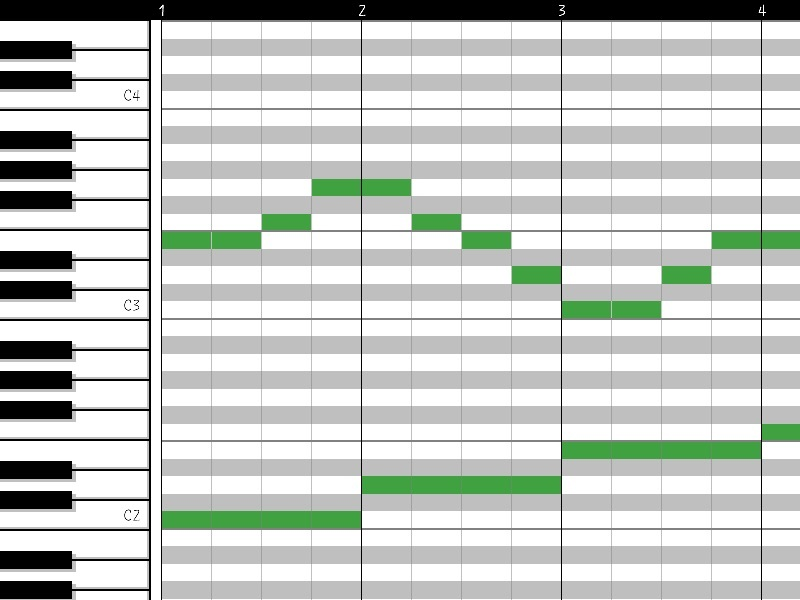
\includegraphics[height=40mm, width=50mm]{z_images/2_midi/exemple_midi_piano.jpg}
	\caption{Exemple évènements avec durée}
\end{figure}
\newpage
Chaque évènement MIDI rassemble un ensemble d’informations sur la hauteur, la durée, le volume, etc… :
\begin{figure}[h]
	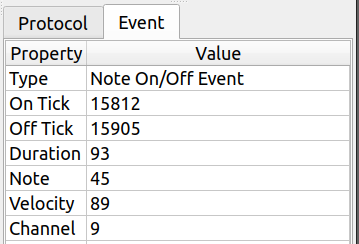
\includegraphics[height=40mm, width=50mm]{z_images/2_midi/representation_numerique_1.png}
	\caption{Critère pour un évènement}
\end{figure}\\
Pour la batterie, les évènements sont considérés sans durée, nous ignorerons donc les offsets (« Off Event »), les « Off Tick » et les « Duration ». Le channel ne nous sera pas utile non-plus.
\textit{Ici, définir Tick et channel.}
Voici un exemple de piano-roll midi pour la batterie :
\begin{figure}[h]
	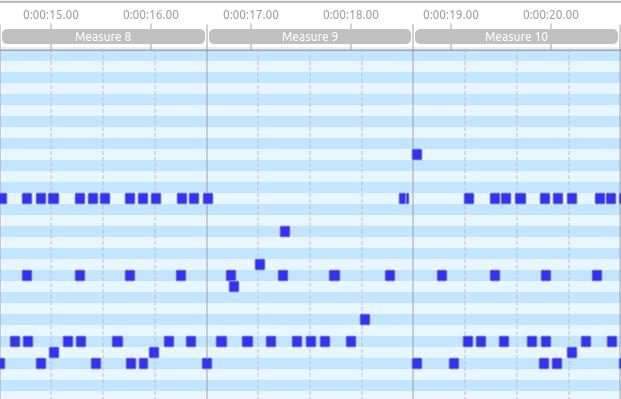
\includegraphics[height=40mm, width=50mm]{z_images/2_midi/representation_numerique_0.png}
	\caption{Exemple évènements sans durée}
\end{figure}\\
On observe que toutes les durées sont identiques.
\subsubsection{La grammaire pondérée}
Système de rythmes préférés.
\subsubsection{Le parsing}
Le parsing du midi donné en input crée une représentation symbolique sous forme d’arbre de rythme.\\
Ici $\Rightarrow$ exemple avec :\\
3bars\_fill\_groove-016.mid $\Rightarrow$ arbre\\
\subsubsection{La séparation des voix}
Plusieurs écritures sont possibles pour un même rythme :
\begin{figure}[h]
	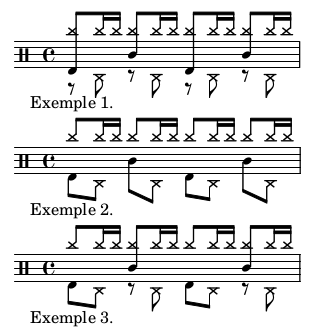
\includegraphics[height=65mm, width=60mm]{z_images/1_description_notation/separation/0_exemples_separation.png}
	\caption{Séparation des voix}
\end{figure}\\
Sur la figure 3.4, il faudra faire un choix entre les exemples 1, 2 et 3 qui sont trois façon d’écrire la même chose. Ce choix se fera en fonction de la lisibilité, de quelles instruments auront des phrasés plus ou moins chargé et/ou variés, auquel cas on les mettra dans une seule voix afin de ne pas charger la partition, etc.
Ainsi l’arbre syntaxique de départ sera divisé en autant d’instruments qui le constituent et les voix seront regroupées de manière cohérentes.
\subsubsection{Les règles de réécriture}
Ici, description basique des règles de réécriture 
\section{Les contributions}
\subsection{Notations, systèmes et réécriture}
\subsubsection{La notation de la batterie}
\textit{Les 3 parties d’une note en général :}
\begin{itemize}
	\item durée
	\item hampe
	\item tête de note (peut aussi indiquer la durée mais en batterie on évitera les blanches, etc.)
\end{itemize}
source : \url{https://fr.wikipedia.org/wiki/Note_de_musique}

\subsubsection{Hauteurs et têtes de notes pour la batterie}
Pour la transcriptions, nous proposons de choisir la base Agostini. La caisse claire centrale sur la portée est aussi centrale sur la batterie est elle est un élément qui conditionne la position des jambes (écart entre les pédales, etc.) ainsi que l’organisation des éléments en hauteur (toms, cymbales, etc.).
On pensera en terme de symétrie la répartition des éléments par rapport au point central que constitue la caisse claire.\\
Cette symétrie s’opère en trois dimensions :
\begin{itemize}
	\item Les hauteurs en terme de fréquences ;
	\item La hauteur physique des éléments :\\
	Du bas vers le haut : pédales, toms et caisse, cymbales
	\item L’ergonomie, qui hiérarchise l’importance des éléments sur la portée (caisse claire au centre, hh-pied et ride sont aux deux extrémités).
\end{itemize}
\begin{figure}[h]
	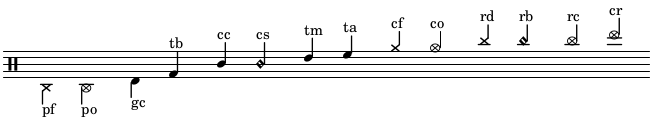
\includegraphics[height=30mm, width=155mm]{z_images/1_description_notation/notes.png}
	\caption{Hauteur et têtes de notes}
\end{figure}
\subsubsection{Les nuances}
\begin{figure}[h]
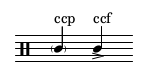
\includegraphics[height=20mm, width=35mm]{z_images/1_description_notation/nuances.png}
\caption{Nuances}
\end{figure}
Bien expliquer les accents, remplacer p et f par g et a\\
$\Rightarrow$ nuance VS articulation\

\subsubsection{Les durées}
Basé sur \cite{jacquemard:hal-01134096} et sur \cite{jacquemard:hal-01403982}\\
Pour la plupart des instruments mélodiques, la liaison et le point sont les deux seules possibilités en cas d’équivalence rythmique pour des notes dont la durée de l’une à l’autre est ininterrompue. Mais puisque les durées des notes n’ont pas d’importance en batterie, l’usage des silences pour combler la distance rythmique entre deux notes devient possible.\\
Ceci pris en compte, et étant donné que les indications de durée dans les têtes de notes ne sont pas pratique en batterie (les symboles « x » des cymbales ne
peuvent pas porter d’indication de durée dans la tête de notes\footnote{Certains logiciels le permettent mais leur lecture reste peu aisée}), l’écriture à l’aide de silences sera privilégiée comme indication de durée sauf dans les cas où cela reste impossible. Ce choix à pour but de n’avoir qu’une manière d’écrire toutes notes, que leurs têtes de notes soit modifiées ou non.\\\\
\textit{Exemple blanche vs noire + soupir}\\

Les cymbales-crash et les ouvertures de charley constituent les seusl cas qui excluent cette option. Le charley car ses ouvertures/fermetures sont presque toujours quantifiées et les cymbales-crash car elles peuvent être arrêtées à la main de manière quantifié aussi mais ce cas est très rare, nous allons donc nous concentrer sur les ouvertures de charley et considérer les crashs comme des événements sans durée.\\
Les fermetures du charley sont notées soit par un silence (correspondant à une fermeture de la pédale), soit par un écrasement de l’ouverture par un autre coup de charley fermé, au pied ou à la main.
\begin{figure}[h]
	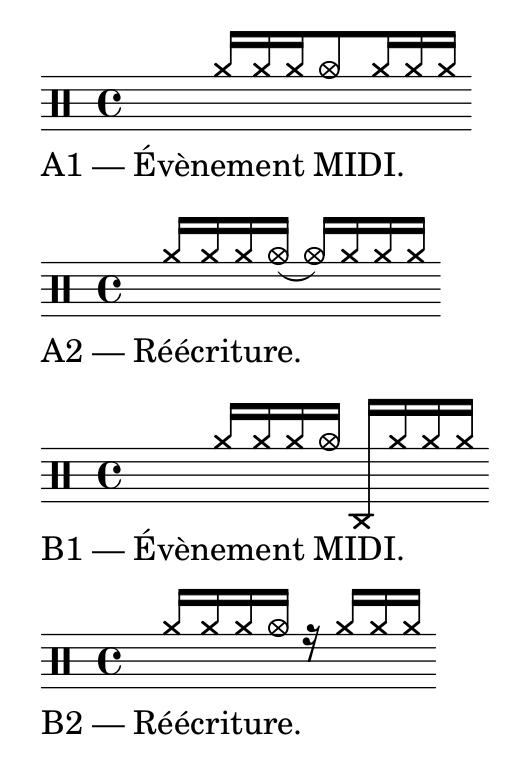
\includegraphics[height=80mm, width=60mm]{z_images/reecriture/exemples_charley_1.png}
	\caption{Durées}
\end{figure} 
\subsection*{La représentation numérique de la batterie}
\subsubsection{Les pitchs}
\begin{table}[h]
	\centering
	\begin{tabular}{|c|c|c|} \hline
		Codes & Instruments & Pitchs \\ \hline
		cf & charley-main-fermé & 22, 42 \\
		co & charley-main-ouvert & 26 \\
		pf & charley-pied-fermé & 44 \\
		rd & ride & 51 \\
		rb & ride-cloche (bell) & 53 \\
		rc & ride-crash & 59 \\
		cr & crash & 55 \\
		cc & caisse-claire & 38, 40 \\
		cs & cross-stick & 37 \\
		ta & tom-alto & 48, 50 \\
		tm & tom-medium & 45, 47 \\
		tb & tom-basse & 43, 58 \\
		gc & grosse-caisse & 36 \\ \hline
	\end{tabular}
	\caption{Pitchs et instruments}
	%	\label{tab:exemple}
\end{table}
Pas de charley pied ouvert…
\subsubsection{La vélocité}
\begin{table}[h]
	\centering
	\begin{tabular}{|c|c|c|c|} \hline
		Codes & Instruments & Pitchs & Vélocité \\ \hline
		cop & charley-main-ouvert & 46 & ? \\ \hline
	\end{tabular}
	\caption{Vélocité et nuances}
\end{table}
Nous ne prendrons en compte la vélocité que pour la cc, les toms et les cymbales jouées aux mains. Les nuances de grosse caisse et charley aux pieds sont le plus souvent insignifiantes, elles ne sont marquées sur le figure qu’à titre indicatif.
Si la vélocité est en dessous de 40, il s’agit de ghost-notes : la tête de note devra être entouré de parenthèses et le suffixe \textit{p (piano)} devra être ajouté au codes de l’instrument. (Voir ccp ci-dessus.)
Si la vélocité est au dessus de 90, il s’agit de notes accentuées : le symbole « > » et le suffixe \textit{f (forte)} devra être ajouté au codes de l’instrument. (Voir ccf ci-dessus.)
Lorsque la vélocité va de 40 à 89, on considèrera le volume comme normal et aucun symbole supplémentaire ne sera ajouté à la note.\\\\

\subsubsection{Les dilemmes}
Le charley de pitch 46 est considéré comme le charley ouvert joué à la main sur le haut de la cymbale mais souvent, ça correspond au geste « tranche-olive » de la baguette lorsque le batteur accentue avec la tranche et joue moins fort avec l’olive sur le plat de la cymbale. Je vais dans un premier temps considérer le pitch comme \textbf{charley-main-ouvert-piano} (ghost-note)
\newpage
\subsubsection{Représentations en arbres}
Voici une représentation de la \textit{partition 3} en arbre de rythme avec les codes de chaque instrument :\\\\
\Tree[ [ [rd\\gc ][ [rd\\pf ][rd ]]]
[ [rd\\cc ][ [rd\\pf ][rd ]]]
[ [rd\\gc ][ [rd\\pf ][rd ]]]
[ [rd\\cc ][ [rd\\pf ][rd ]]] ]\\\\\\
Ci-dessous, le même arbre dont les codes des instruments sont remplacés par leurs données midi respectives :\\\\
\Tree[ [ [51\\36 ][ [51\\44 ][51 ]]]
[ [51\\38 ][ [51\\44 ][51 ]]]
[ [51\\36 ][ [51\\44 ][51 ]]]
[ [51\\38 ][ [51\\44 ][51 ]]] ]\\\\\\
Cet arbre représente un rythme unique dont les possiblités de notation sur une partition sont théoriquement multiples.(Voir \textit{partition 3}).
\subsection*{Les systèmes}
\subsubsection{Définition}

Un système est la combinaison d’un ou plusieurs éléments qui jouent un rythme en boucle (motif) et d’un autre élément qui joue un texte rythmique variable mais respectant les règles propre au système (gamme).\\

Système = motif + gamme/texte\\
motif = rythmes coordonnés joués avec 2 ou 3 membres en boucle (reparti sur 1 ou 2 voix)\\
gamme/texte = rythme irrégulier joué avec un seul membre sur le motif (Réparti sur 1 voix). La gamme d’un système considère l’ensemble des combinaisons que le batteur pourrait rencontrer en interprétant un texte rythmique à l’aide du système.\\

Nous partirons de propositions génériques de systèmes (environs trois systèmes dans différents styles de batterie) que nous tenterons de détecter dans le jeu de données groove.\\

Quatre systèmes standards :
\begin{itemize}
	\item binaire
	\item ternaire (shuffle, afro, rock)
	\item jazz
	\item afro-cubain\\
\end{itemize}

Nous travaillerons aussi sur la détection de répétitions sur plusieurs mesures afin de pouvoir corriger des erreurs sur une des mesures qui aurait dû être identique aux autres mais qui présente des différences.

\subsubsection{Utilité}
\begin{itemize}
	\item Séparation des voix
	\item Définir une métrique
	\item Conditionner des règles spécifiques de réécriture
\end{itemize}

Créer un ensemble de systèmes :
\begin{itemize}
	\item 4/4 binaire FAIT
	\item jazz vs ternaire(12/8) EN COURS…
	\item afro-cubain
	\item Tout transcrire avec lilypond et en arbres d’analyse syntaxique.
	\item Créer les arbres de voix séparées.
	\item Écrire les règles de réécriture.
	\item Créer les arbres de voix séparées simplifiés (rewriting).\\	
\end{itemize}

Pour la \textbf{séparation des voix} et la \textbf{définition des métriques}, nous nous intéresserons principalement à la partie \textit{motif} des systèmes qui seront présentés. La partie \textit{texte} nous intéressera plus pour les \textbf{combinaisons de réécritures}.
\newpage
\subsubsection{Pour la séparation des voix}
\textbf{Motif 4-4 binaire}\\\\
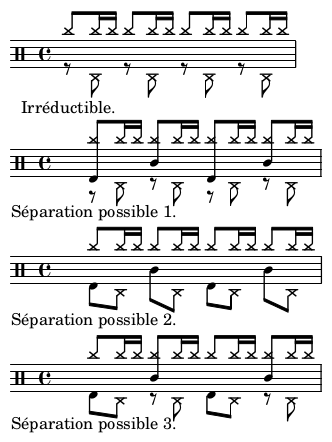
\includegraphics[height=60mm, width=40mm]{z_images/1_description_notation/separation/1_separation_4-4_binaire.png}\\\\
Ici, le système est construit sur un modèle rock en 4/4 : after-beat sur les 2 et 4 avec un choix de répartition des cymbales type fast-jazz. Le système est constitué par défaut du motif ride/ch-pf/cc et d’un texte joué à la grosse-caisse. La troisième séparation proposée est privilégiée car elle répartit selon 2 voix, une voix pour les mains (ride + cc) et une voix pour les pieds (ch-pf + gc). Ce choix paraît plus équilibré car deux instruments sont utilisés par voix et plus logique pour le lecteur puisque les mains sont en haut et les pieds en bas.\\
%D’autres choix d’écriture auraient été possibles :
%\begin{itemize}
%	\item Toutes les hampes en haut ;
%	\item Combinaison motif 1 et 2 en donnant 2 directions aux hampes de la cc).\\
%\end{itemize}

\textbf{Motif 4-4 jazz}\\\\
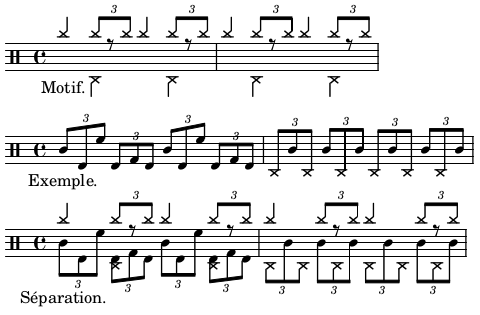
\includegraphics[height=45mm, width=60mm]{z_images/1_description_notation/separation/2_separation_4-4_jazz.png}\\\\
Dans la plupart des méthodes, le charley n’est pas écrit car considéré comme évident en jazz traditionnel. Ce qui facilite grandement l’écriture : la ride et les crash sur la voix du haut et le reste sur la voix du bas. Ici, le partie prit et de tout écrire. Dans l’exemple ci-dessus, les mesures 1 et 2 combinées avec le \textit{motif} de la première ligne, sont des cas typiques de la batterie jazz. Tout mettre sur la voix haute serait surchargé. De plus, la grosse caisse entre très souvent dans le flot des combinaisons de toms et de caisse claire et son écriture séparée serait inutilement compliquée et peu intuitive pour le lecteur. Le choix de séparation sera donc de laisser les cymbales en haut et toms, caisse-claire, grosse-caisse et pédale de charley en bas.
\newpage

\textbf{Système 4-4 afro-cubain}\\\\
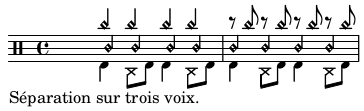
\includegraphics[height=25mm, width=80mm]{z_images/1_description_notation/separation/3_separation_afro-cubain.png}\\\\

\subsubsection{Pour la reconnaissance de la métrique}
\textit{\textbf{12/8 vs 4/4 ternaire}}\\\\
\textbf{Motif 12/8}\\\\
%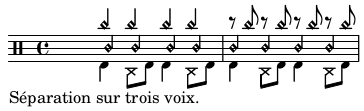
\includegraphics[height=30mm, width=100mm]{z_images/1_description_notation/separation/separation_2.png}\\\\

\subsubsection{Pour les règles de réécriture}
Les textes qui accompagnent les motifs étayent toutes les combinaisons d’un systèmes. 
\newpage

%\subsubsection{Construction des systèmes pour les expérimentations}
\subsubsection{La réécriture des évènements MIDI pour la batterie}



\textbf{Exemples à écrire en arbre :}\\
\begin{itemize}
	\item 
	SI (pas pf) ET (note sur un temps suivie de note en l’air) :\\
	$\Rightarrow$ (Temps1 : Note pertinente) + (Temps2 : Silence pertinent + Note pertinente.)\\
	\item
	Si (po ou co) déborde sur le temps suivant :\\
	$\Rightarrow$ Liaison car marchera dans tous les cas même la où le point ne marchera pas (voir A2).\\
	\item
	Une blanche sera écrite noir + soupir.\\\\
\end{itemize}
\subsubsection{Les régles de réécriture}
~~\\
\Tree[.$\frac{2}{8}$ [.x ][.tie ]]\Tree[.2/8 [.x ]]\\\\\\
\Tree[.1/4 [.x ][.tie ]]\Tree[.1/4 [.x ][.r ]]\\\\\\

\section{Conclusion}
Bilan sur les différentes méthodes employées et la contribution que cela représente.

\chapter{Expérimentations et résultats}
\label{chap:08_experimentations_et_resultats}
\minitoc
\section{Introduction}
Dans ce chapitre, nous présenterons le corpus, les expérimentations et les différents choix effectués pour les tests.
\section{Le corpus}
\textbf{groove MIDI dataset}\\
\url{https://magenta.tensorflow.org/datasets/groove}\\\\
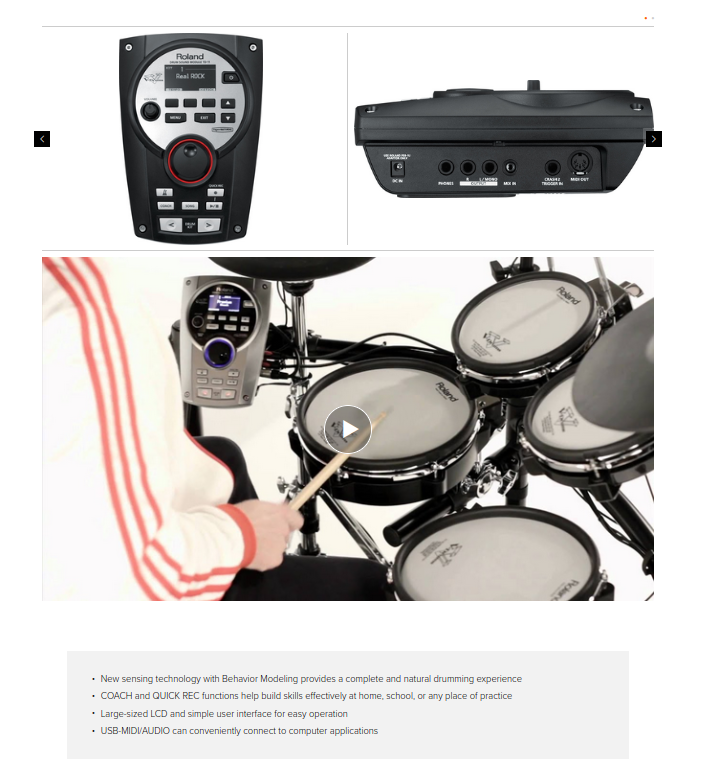
\includegraphics[height=60mm, width=60mm]{z_images/3_groove/roland_TD11.png}\\
Des batteurs pro ont été engagés pour jouer sur un roland td-11\\\\
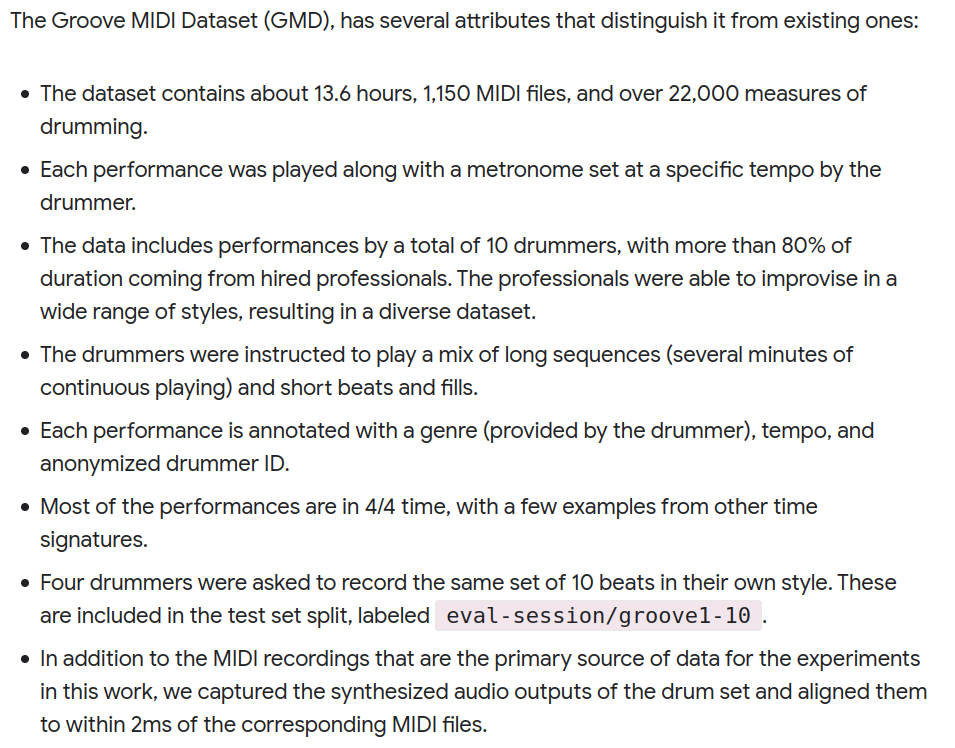
\includegraphics[height=80mm, width=110mm]{z_images/3_groove/dataset_how.png}\newpage{}
\textbf{Les métadatas :}\\\\
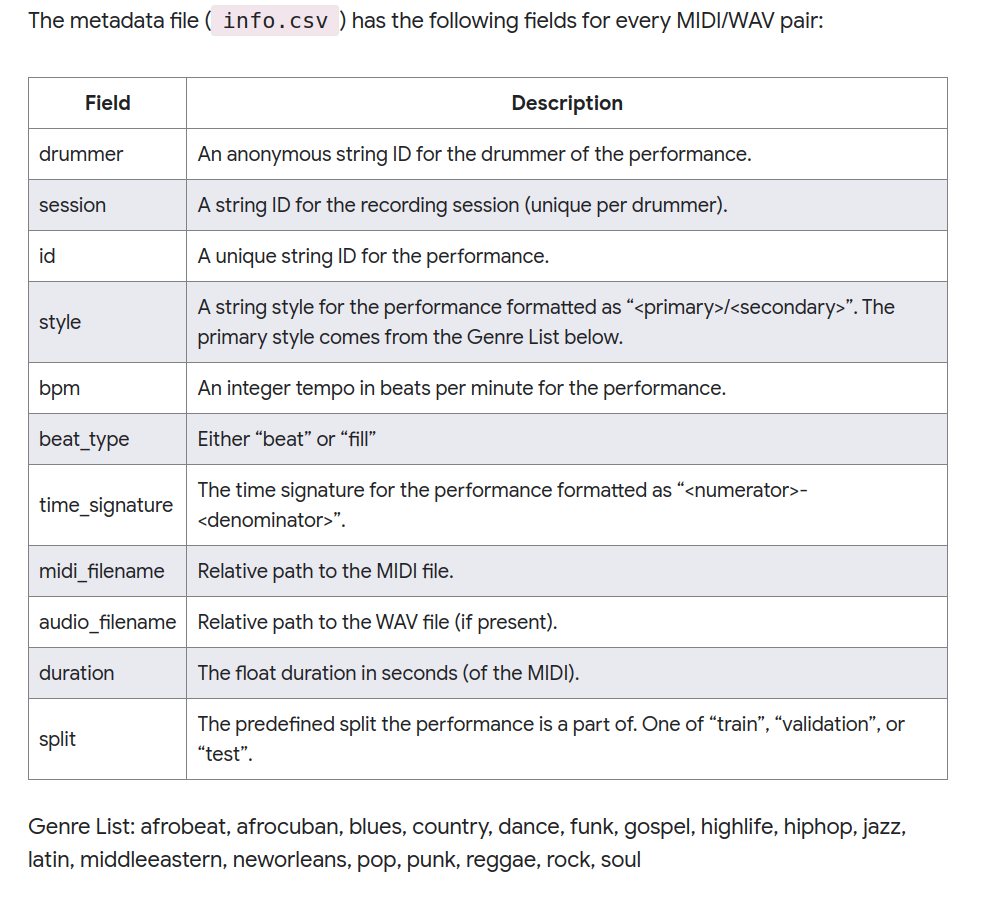
\includegraphics[height=85mm, 
width=100mm]{z_images/3_groove/csv_metadata_struct.png}\\
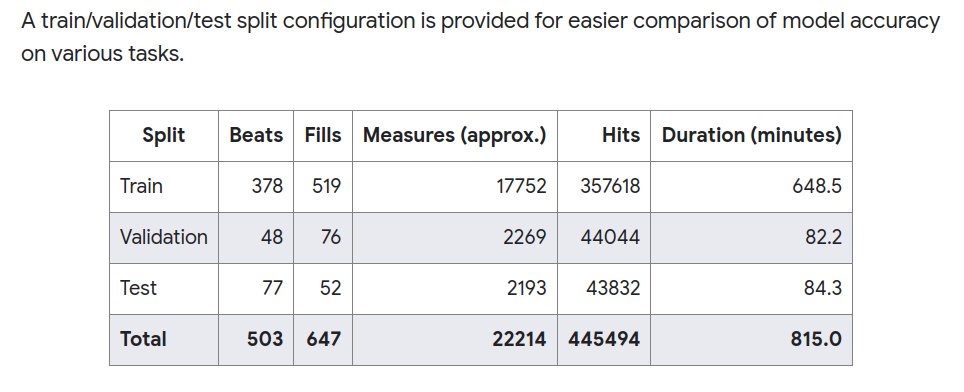
\includegraphics[height=50mm, width=120mm]{z_images/3_groove/train_validation_test.png}\\
Détails (entre autres tensorflow avec le dataset) à :
\url{https://magenta.tensorflow.org/datasets/groove#license}\\
écouter le dataset groove
\newpage
\section{Les contributions}
\subsection{comparaisons de transcriptions}
\textit{drummer\_01/session3 — 10\_rock-folk\_90\_beat\_4-4}\\\\
Fichier midi vers partition avec musescore $\Rightarrow$ Transcription manuelle\\
\includegraphics[height=20mm, width=50mm]{z_images/transcriptions_manuelles/0_prise_en_main/0_tests_drummer_01__session3/musescore_0.png}\ \ \ \ 
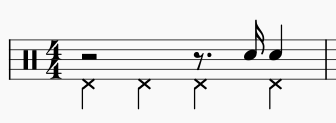
\includegraphics[height=20mm, width=55mm]{z_images/transcriptions_manuelles/0_prise_en_main/0_tests_drummer_01__session3/manuel_0.png}
\textit{drummer\_01/session3 — 10\_rock-folk\_90\_beat\_4-4}\\\\
Fichier midi vers partition avec musescore $\Rightarrow$ Transcription manuelle\\
\includegraphics[height=20mm, width=50mm]{z_images/transcriptions_manuelles/0_prise_en_main/0_tests_drummer_01__session3/musescore_0.png}\ \ \ \ 
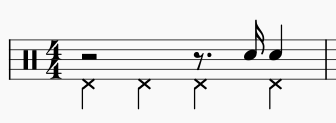
\includegraphics[height=20mm, width=55mm]{z_images/transcriptions_manuelles/0_prise_en_main/0_tests_drummer_01__session3/manuel_0.png}
\begin{itemize}
	\item Erreur d’indication de mesure ;
	\item Mauvaise transcription d’une noire.\\
\end{itemize}
La noire du 4ème temps se retrouve sur le premier temps de la mesure suivante et elle se transforme en un triolet de double croches dont seules les deux premières seraient jouées.\\\\
\textit{drummer\_01/session3 — 10\_rock-folk\_90\_beat\_4-4}\\\\
Fichier midi vers partition avec musescore $\Rightarrow$ Transcription manuelle\\
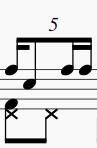
\includegraphics[height=20mm, width=15mm]{z_images/transcriptions_manuelles/0_prise_en_main/0_tests_drummer_01__session3/musescore_1.png}\ \ \ \ 
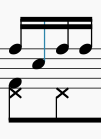
\includegraphics[height=20mm, width=15mm]{z_images/transcriptions_manuelles/0_prise_en_main/0_tests_drummer_01__session3/manuel_1.png}\\
\begin{itemize}
	\item Erreur de quantification : les doubles croches ont été interprétées en quintolet;\\
\end{itemize}
drummer\_01/session3 — 2\_jazz-swing\_185\_beat\_4-4\\\\
Fichier midi vers partition avec musescore $\Rightarrow$ Transcription manuelle\\
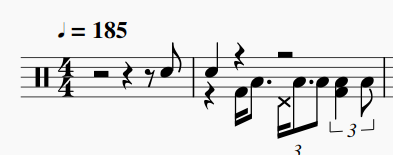
\includegraphics[height=25mm, width=60mm]{z_images/transcriptions_manuelles/0_prise_en_main/0_tests_drummer_01__session3/musescore_2.png}\ \ \ \ 
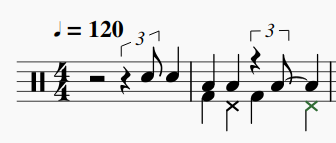
\includegraphics[height=25mm, width=55mm]{z_images/transcriptions_manuelles/0_prise_en_main/0_tests_drummer_01__session3/manuel_2.png}
\begin{itemize}
	\item L’indication de mesure est correcte mais tout a été décalé d’un temps car la première noire sur la caisse claire est jouée sur le 4ème temps et non sur le premier temps de la deuxième mesure comme l’indique la transcription de musescore.
	\item Les toms basses des 1er et 2ème temps de la mesure musescore auraient dû être sur les temps et non décalés d’une double croche vers la droite.\\
\end{itemize}
drummer\_01/session1 — 1\_funk\_80\_beat\_4-4\\\\
Fichier midi vers partition avec musescore $\Rightarrow$ Transcription manuelle\\
\includegraphics[height=25mm, width=40mm]{z_images/transcriptions_manuelles/0_prise_en_main/1_drummer_01__session1/musescore_0.png}\ \ \ \ 
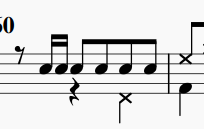
\includegraphics[height=25mm, width=40mm]{z_images/transcriptions_manuelles/0_prise_en_main/1_drummer_01__session1/Manuelle_0.png}
\begin{itemize}
	\item On dirait que lorsque certaines notes sont proches, elles se resserrent et suppriment celles qui aurait dû être sur le temps.\\
	\item Erreur d’indication de mesure ;
	\item Mauvaise transcription d’une noire.\\
\end{itemize}
La noire du 4ème temps se retrouve sur le premier temps de la mesure suivante et elle se transforme en un triolet de double croches dont seules les deux premières seraient jouées.\\\\
\textit{drummer\_01/session3 — 10\_rock-folk\_90\_beat\_4-4}\\\\
Fichier midi vers partition avec musescore $\Rightarrow$ Transcription manuelle\\
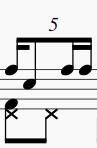
\includegraphics[height=20mm, width=15mm]{z_images/transcriptions_manuelles/0_prise_en_main/0_tests_drummer_01__session3/musescore_1.png}\ \ \ \ 
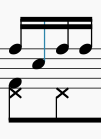
\includegraphics[height=20mm, width=15mm]{z_images/transcriptions_manuelles/0_prise_en_main/0_tests_drummer_01__session3/manuel_1.png}\\
\begin{itemize}
	\item Erreur de quantification : les doubles croches ont été interprétées en quintolet;\\
\end{itemize}
drummer\_01/session3 — 2\_jazz-swing\_185\_beat\_4-4\\\\
Fichier midi vers partition avec musescore $\Rightarrow$ Transcription manuelle\\
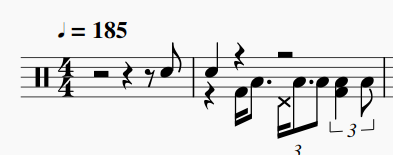
\includegraphics[height=25mm, width=60mm]{z_images/transcriptions_manuelles/0_prise_en_main/0_tests_drummer_01__session3/musescore_2.png}\ \ \ \ 
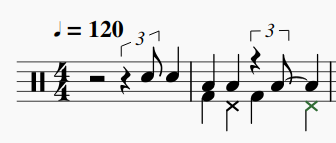
\includegraphics[height=25mm, width=55mm]{z_images/transcriptions_manuelles/0_prise_en_main/0_tests_drummer_01__session3/manuel_2.png}
\begin{itemize}
	\item L’indication de mesure est correcte mais tout a été décalé d’un temps car la première noire sur la caisse claire est jouée sur le 4ème temps et non sur le premier temps de la deuxième mesure comme l’indique la transcription de musescore.
	\item Les toms basses des 1er et 2ème temps de la mesure musescore auraient dû être sur les temps et non décalés d’une double croche vers la droite.\\
\end{itemize}
drummer\_01/session1 — 1\_funk\_80\_beat\_4-4\\\\
Fichier midi vers partition avec musescore $\Rightarrow$ Transcription manuelle\\
\includegraphics[height=25mm, width=40mm]{z_images/transcriptions_manuelles/0_prise_en_main/1_drummer_01__session1/musescore_0.png}\ \ \ \ 
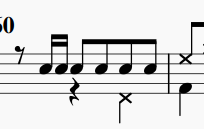
\includegraphics[height=25mm, width=40mm]{z_images/transcriptions_manuelles/0_prise_en_main/1_drummer_01__session1/Manuelle_0.png}
\begin{itemize}
	\item On dirait que lorsque certaines notes sont proches, elles se resserrent et suppriment celles qui aurait dû être sur le temps.\\
\end{itemize}
%drummer\_01/session1 — 1\_funk\_80\_beat\_4-4\\
%Fichier midi vers partition avec musescore :\\\\
%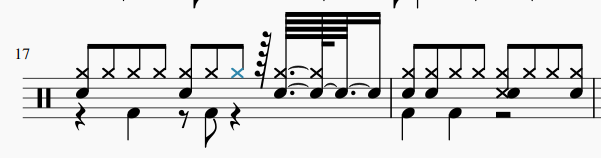
\includegraphics[height=25mm, width=80mm]{z_images/transcriptions_manuelles/0_prise_en_main/1_drummer_01__session1/MuseScore_1.png} \\\\
%Transcription manuelle :\\
%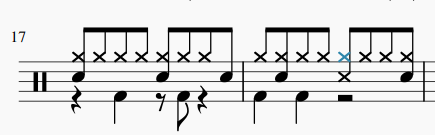
\includegraphics[height=20mm, width=65mm]{z_images/transcriptions_manuelles/0_prise_en_main/1_drummer_01__session1/Manuelle_1.png} \\
%\begin{itemize}
%	\item La caisse claire de la 2ème croche du 4ème temps de la 1ère mesure se transforme en une combinaison de quadruple/quintuple/double croches liées qui commence par un soupir et finit en débordant sur le premier temps de la mesure suivante. 
%\end{itemize}
\subsubsection{Exemple avec des flas}
%Des exemples de notation flas tom/caisse-claire existent dans des partitions récentes (rythmique binaire J.-F. Juskowiak).\\
%$\Rightarrow$ Ils faudra donc les prendre en compte dans les comparaisons de transcriptions.
Fichier midi vers partition avec musescore :\\
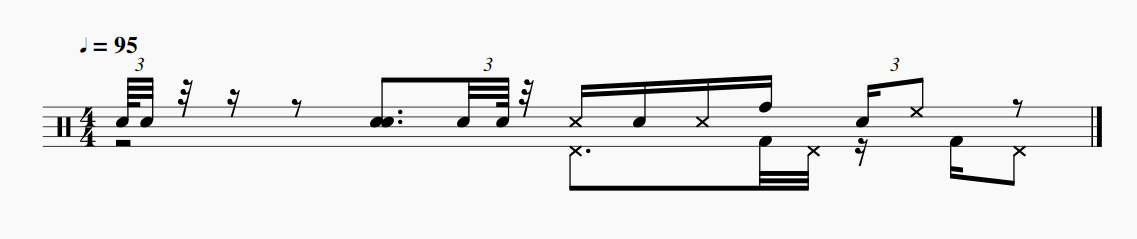
\includegraphics[height=30mm, width=120mm]{z_images/transcriptions_manuelles/1_transcriptions_flas/124_funk_95_fill_4-4_0.png}\\
Transcription manuelle :\\
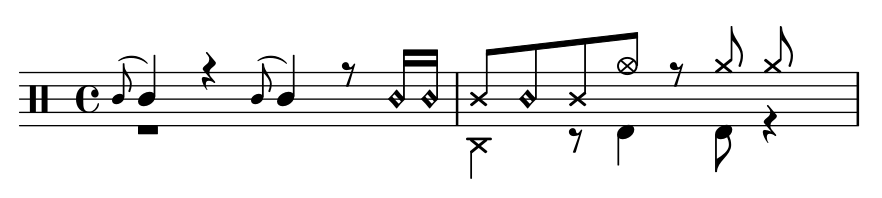
\includegraphics[height=20mm, width=90mm]{z_images/transcriptions_manuelles/1_transcriptions_flas/124_funk_95_fill_4-4_1_.png}\\
\subsection{Les tests unitaires}
\section{Choix pour les tests}
\subsection{Expérience 1 - 4/4 binaire}
\subsubsection{Partition de référence pour l’ouput}
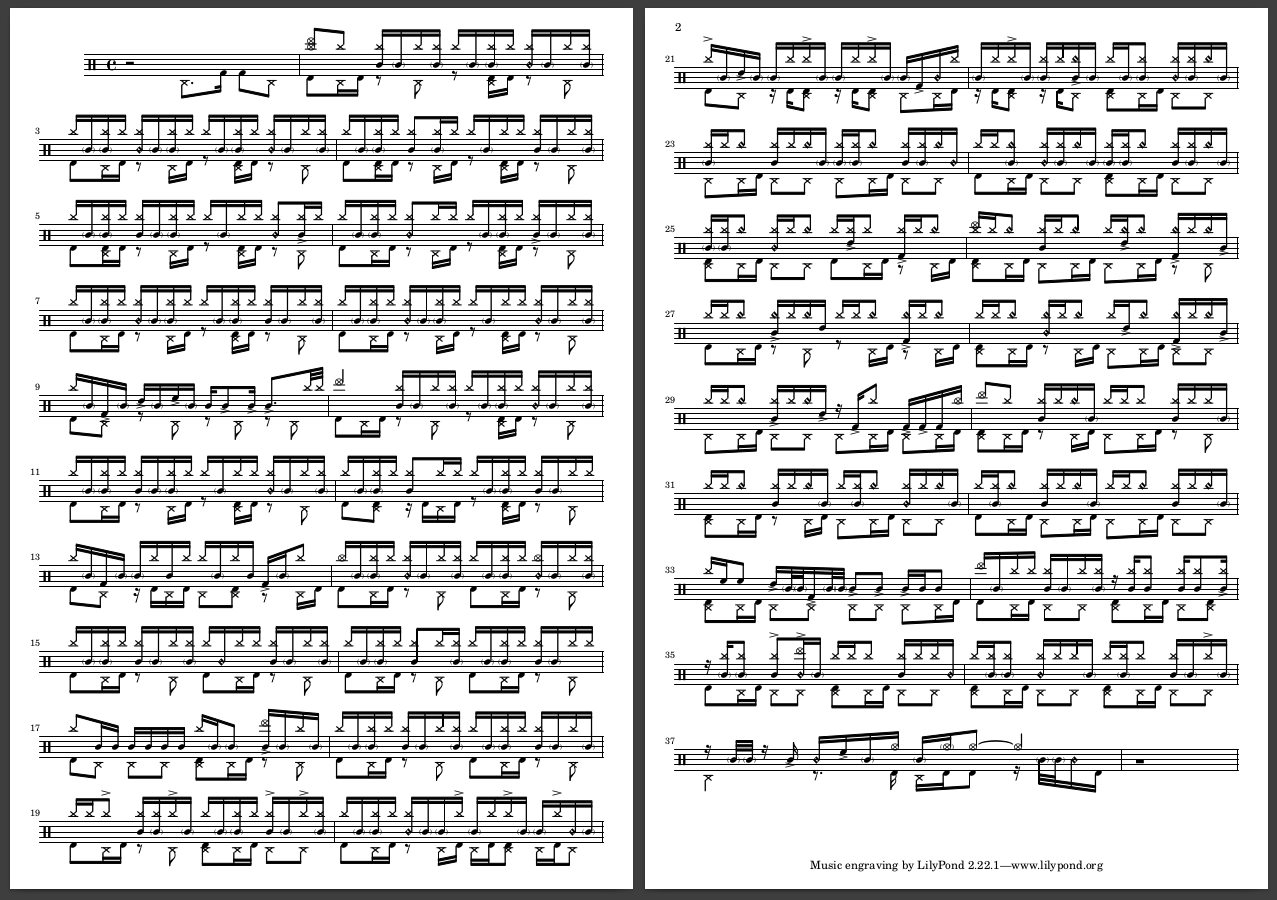
\includegraphics[height=120mm, width=160mm]{z_images/4_experimentations/experience_1/partition.png}
\subsubsection{Systèmes recherchés}
Textes :\\\\
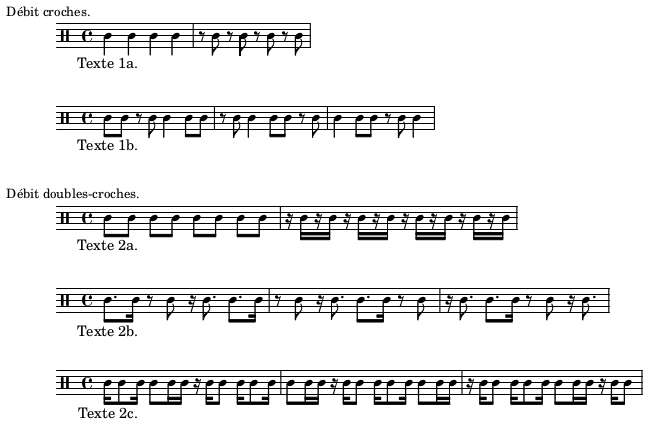
\includegraphics[height=70mm, width=95mm]{z_images/1_description_notation/systemes/0_textes_4-4_binaires.png}\\
Motifs :\\\\
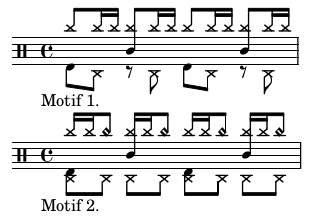
\includegraphics[height=30mm, width=40mm]{z_images/1_description_notation/systemes/1_motifs_4-4_binaires.png}\\\\
Systèmes résultants :\\\\
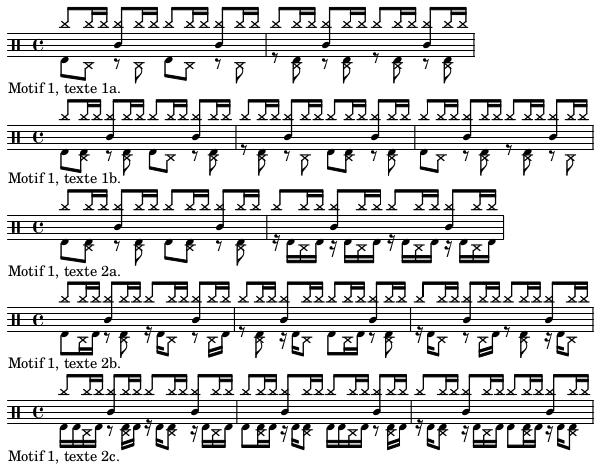
\includegraphics[height=75mm, width=85mm]{z_images/4_experimentations/experience_1/systeme_recherche_1.png}
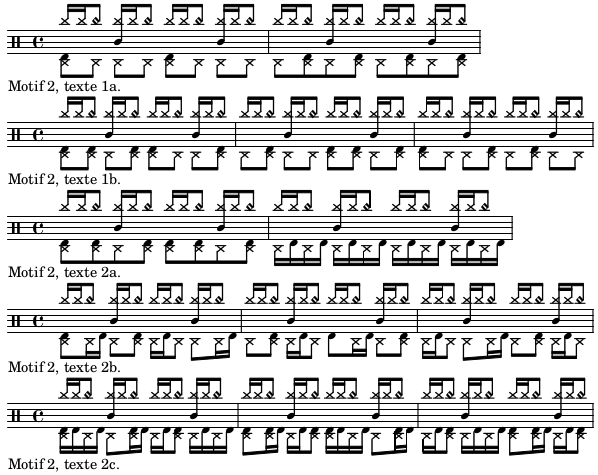
\includegraphics[height=75mm, width=85mm]{z_images/4_experimentations/experience_1/systeme_recherche_2.png}


\subsubsection{Représentation des systèmes en arbres de rythmes}

\resizebox{500pt}{!} {
	\Tree[.Motif\ 1\ +\ Texte\ 1a
	[.Mesure\ 1
	[.Temps\ 1 [rd\\bd ][ [rd\\pf ][rd ]]]
	[.Temps\ 2 [rd\\cc ][ [rd\\pf ][rd ]]]
	[.Temps\ 3 [rd\\bd ][ [rd\\pf ][rd ]]]
	[.Temps\ 4 [rd\\cc ][ [rd\\pf ][rd ]]] ]
	[.Mesure\ 2
	[.Temps\ 1 [rd ][ [rd\\bd\\pf ][rd ]]]
	[.Temps\ 2 [rd\\cc ][ [rd\\bd\\pf ][rd ]]]
	[.Temps\ 3 [rd ][ [rd\\bd\\pf ][rd ]]]
	[.Temps\ 4 [rd\\cc ][ [rd\\bd\\pf ][rd ]]] ]]}\\

\resizebox{500pt}{!} {
	\Tree[.Motif\ 1\ +\ Texte\ 1b
	[.Mesure\ 1
	[.Temps\ 1 [rd\\bd ][ [rd\\bd\\pf ][rd ]]]
	[.Temps\ 2 [rd\\cc ][ [rd\\bd\\pf ][rd ]]]
	[.Temps\ 3 [rd\\bd ][ [rd\\pf ][rd ]]]
	[.Temps\ 4 [rd\\cc ][ [rd\\bd\\pf ][rd ]]] ]
	[.Mesure\ 2
	[.Temps\ 1 [rd ][ [rd\\bd\\pf ][rd ]]]
	[.Temps\ 2 [rd\\cc ][ [rd\\pf ][rd ]]]
	[.Temps\ 3 [rd\\bd ][ [rd\\bd\\pf ][rd ]]]
	[.Temps\ 4 [rd\\cc ][ [rd\\bd\\pf ][rd ]]] ]
	[.Mesure\ 3
	[.Temps\ 1 [rd\\bd ][ [rd\\pf ][rd ]]]
	[.Temps\ 2 [rd\\cc ][ [rd\\bd\\pf ][rd ]]]
	[.Temps\ 3 [rd ][ [rd\\bd\\pf ][rd ]]]
	[.Temps\ 4 [rd\\cc ][ [rd\\pf ][rd ]]] ]]}\\

\resizebox{500pt}{!} {
	\Tree[.Motif\ 1\ +\ Texte\ 2a
	[.Mesure\ 1
	[.Temps\ 1 [rd\\bd ][ [rd\\bd\\pf ][rd ]]]
	[.Temps\ 2 [rd\\cc ][ [rd\\bd\\pf ][rd ]]]
	[.Temps\ 3 [rd\\bd ][ [rd\\bd\\pf ][rd ]]]
	[.Temps\ 4 [rd\\cc ][ [rd\\bd\\pf ][rd ]]] ]
	[.Mesure\ 2
	[.Temps\ 1 [rd ][bd ][rd\\pf ][rd\\bd ]]
	[.Temps\ 2 [rd\\cc ][bd ][rd\\pf ][rd\\bd ]]
	[.Temps\ 3 [rd ][bd ][rd\\pf ][rd\\bd ]]
	[.Temps\ 4 [rd\\cc ][bd ][rd\\pf ][rd\\bd ]] ]]}\\

\resizebox{500pt}{!} {
	\Tree[.Motif\ 1\ +\ Texte\ 2b
	[.Mesure\ 1
	[.Temps\ 1 [rd\\bd ][ [rd\\pf ][rd\\bd ]]]
	[.Temps\ 2 [rd\\cc ][ [rd\\bd\\pf ][rd ]]]
	[.Temps\ 3 [rd ][bd ][rd\\pf ][rd ]]
	[.Temps\ 4 [rd\\cc ][ [rd\\pf ][rd\\bd ]]] ]
	[.Mesure\ 2
	[.Temps\ 1 [rd\\ ][ [rd\\bd\\pf ][rd ]]]
	[.Temps\ 2 [rd\\cc ][bd ][rd\\pf ][rd ]]
	[.Temps\ 3 [rd\\bd ][ [rd\\pf ][rd\\bd ]]]
	[.Temps\ 4 [rd\\cc ][ [rd\\bd\\pf ][rd ]]] ]
	[.Mesure\ 3
	[.Temps\ 1 [rd ][bd ][rd\\pf ][rd ]]
	[.Temps\ 2 [rd\\cc ][ [rd\\pf ][rd\\bd ]]]
	[.Temps\ 3 [rd ][ [rd\\bd\\pf ][rd ]]]
	[.Temps\ 4 [rd\\cc ][bd ][rd\\pf ][rd ]]] ] }\\

\resizebox{500pt}{!} {
	\Tree[.Motif\ 1\ +\ Texte\ 2c
	[.Mesure\ 1
	[.Temps\ 1 [rd\\bd ][bd ][rd\\pf ][rd\\bd ]]
	[.Temps\ 2 [rd\\cc ][ [rd\\bd\\pf ][rd\\bd ]]]
	[.Temps\ 3 [rd ][bd ][rd\\bd\\pf ][rd ]]
	[.Temps\ 4 [rd\\cc ][bd ][rd\\pf ][rd\\bd ]] ]
	[.Mesure\ 2
	[.Temps\ 1 [rd\\bd ][ [rd\\bd\\pf ][rd\\bd ]]]
	[.Temps\ 2 [rd\\cc ][bd ][rd\\bd\\pf ][rd ]]
	[.Temps\ 3 [rd\\bd ][bd ][rd\\pf ][rd\\bd ]]
	[.Temps\ 4 [rd\\cc ][ [rd\\bd\\pf ][rd\\bd ]]] ]
	[.Mesure\ 3
	[.Temps\ 1 [rd ][bd ][rd\\bd\\pf ][rd ]]
	[.Temps\ 2 [rd\\cc ][bd ][rd\\pf ][rd\\bd ]]
	[.Temps\ 3 [rd\\bd ][ [rd\\bd\\pf ][rd\\bd ]]]
	[.Temps\ 4 [rd\\cc ][bd ][rd\\bd\\pf ][rd ]]] ] }\\\\

\subsubsection{Séparation des voix}
Motif\ 1\ +\ Texte\ 1a\\\\
\textit{Voix haute}\\
\resizebox{500pt}{!} {
	\Tree[.Motif\ 1\ +\ Texte\ 1a
	[.Mesure\ 1
	[.Temps\ 1 [rd ][ [rd ][rd ]]]
	[.Temps\ 2 [rd\\cc ][ [rd ][rd ]]]
	[.Temps\ 3 [rd ][ [rd ][rd ]]]
	[.Temps\ 4 [rd\\cc ][ [rd ][rd ]]] ]
	[.Mesure\ 2
	[.Temps\ 1 [rd ][ [rd ][rd ]]]
	[.Temps\ 2 [rd\\cc ][ [rd ][rd ]]]
	[.Temps\ 3 [rd ][ [rd ][rd ]]]
	[.Temps\ 4 [rd\\cc ][ [rd ][rd ]]] ]]}\\

\textit{Voix basse}\\
\resizebox{500pt}{!} {
	\Tree[.Motif\ 1\ +\ Texte\ 1a
	[.Mesure\ 1
	[.Temps\ 1 [bd ][ [pf ][t ]]]
	[.Temps\ 2 [t ][ [pf ][t ]]]
	[.Temps\ 3 [bd ][ [pf ][t ]]]
	[.Temps\ 4 [t ][ [pf ][t ]]] ]
	[.Mesure\ 2
	[.Temps\ 1 [t ][ [bd\\pf ][t ]]]
	[.Temps\ 2 [t ][ [bd\\pf ][t ]]]
	[.Temps\ 3 [t ][ [bd\\pf ][t ]]]
	[.Temps\ 4 [t ][ [bd\\pf ][t ]]] ]]}\\

Motif\ 1\ +\ Texte\ 1b\\\\
\textit{Voix haute}\\
\resizebox{500pt}{!} {
	\Tree[.Motif\ 1\ +\ Texte\ 1b
	[.Mesure\ 1
	[.Temps\ 1 [rd ][ [rd ][rd ]]]
	[.Temps\ 2 [rd\\cc ][ [rd ][rd ]]]
	[.Temps\ 3 [rd ][ [rd ][rd ]]]
	[.Temps\ 4 [rd\\cc ][ [rd ][rd ]]] ]
	[.Mesure\ 2
	[.Temps\ 1 [rd ][ [rd ][rd ]]]
	[.Temps\ 2 [rd\\cc ][ [rd ][rd ]]]
	[.Temps\ 3 [rd ][ [rd ][rd ]]]
	[.Temps\ 4 [rd\\cc ][ [rd ][rd ]]] ]
	[.Mesure\ 3
	[.Temps\ 1 [rd ][ [rd ][rd ]]]
	[.Temps\ 2 [rd\\cc ][ [rd ][rd ]]]
	[.Temps\ 3 [rd ][ [rd ][rd ]]]
	[.Temps\ 4 [rd\\cc ][ [rd ][rd ]]] ]]}\\

\textit{Voix basse}\\
\resizebox{500pt}{!} {
	\Tree[.Motif\ 1\ +\ Texte\ 1b
	[.Mesure\ 1
	[.Temps\ 1 [bd ][ [bd\\pf ][t ]]]
	[.Temps\ 2 [t ][ [bd\\pf ][t ]]]
	[.Temps\ 3 [bd ][ [pf ][t ]]]
	[.Temps\ 4 [t ][ [bd\\pf ][t ]]] ]
	[.Mesure\ 2
	[.Temps\ 1 [t ][ [bd\\pf ][t ]]]
	[.Temps\ 2 [t ][ [pf ][t ]]]
	[.Temps\ 3 [bd ][ [bd\\pf ][t ]]]
	[.Temps\ 4 [t ][ [bd\\pf ][t ]]] ]
	[.Mesure\ 3
	[.Temps\ 1 [bd ][ [pf ][t ]]]
	[.Temps\ 2 [t ][ [bd\\pf ][t ]]]
	[.Temps\ 3 [t ][ [bd\\pf ][t ]]]
	[.Temps\ 4 [t ][ [pf ][t ]]] ]]}\\

Motif\ 1\ +\ Texte\ 2a\\\\
\textit{Voix haute}\\
\resizebox{500pt}{!} {
	\Tree[.Motif\ 1\ +\ Texte\ 2a
	[.Mesure\ 1
	[.Temps\ 1 [rd ][ [rd ][rd ]]]
	[.Temps\ 2 [rd\\cc ][ [rd ][rd ]]]
	[.Temps\ 3 [rd ][ [rd ][rd ]]]
	[.Temps\ 4 [rd\\cc ][ [rd ][rd ]]] ]
	[.Mesure\ 2
	[.Temps\ 1 [rd ][t ][rd ][rd ]]
	[.Temps\ 2 [rd\\cc ][t ][rd ][rd ]]
	[.Temps\ 3 [rd ][t ][rd ][rd ]]
	[.Temps\ 4 [rd\\cc ][t ][rd ][rd ]] ]]}\\

\textit{Voix basse}\\
\resizebox{500pt}{!} {
	\Tree[.Motif\ 1\ +\ Texte\ 2a
	[.Mesure\ 1
	[.Temps\ 1 [bd ][ [bd\\pf ][t ]]]
	[.Temps\ 2 [t ][ [bd\\pf ][t ]]]
	[.Temps\ 3 [bd ][ [bd\\pf ][t ]]]
	[.Temps\ 4 [t ][ [bd\\pf ][t ]]] ]
	[.Mesure\ 2
	[.Temps\ 1 [t ][bd ][pf ][bd ]]
	[.Temps\ 2 [t ][bd ][pf ][bd ]]
	[.Temps\ 3 [t ][bd ][pf ][bd ]]
	[.Temps\ 4 [t ][bd ][pf ][bd ]] ]]}\\

Motif\ 1\ +\ Texte\ 2b\\\\
\textit{Voix haute}\\
\resizebox{500pt}{!} {
	\Tree[.Motif\ 1\ +\ Texte\ 2b
	[.Mesure\ 1
	[.Temps\ 1 [rd ][ [rd ][rd ]]]
	[.Temps\ 2 [rd\\cc ][ [rd ][rd ]]]
	[.Temps\ 3 [rd ][t ][rd ][rd ]]
	[.Temps\ 4 [rd\\cc ][ [rd ][rd ]]] ]
	[.Mesure\ 2
	[.Temps\ 1 [rd\\ ][ [rd ][rd ]]]
	[.Temps\ 2 [rd\\cc ][t ][rd ][rd ]]
	[.Temps\ 3 [rd ][ [rd ][rd ]]]
	[.Temps\ 4 [rd\\cc ][ [rd ][rd ]]] ]
	[.Mesure\ 3
	[.Temps\ 1 [rd ][t ][rd ][rd ]]
	[.Temps\ 2 [rd\\cc ][ [rd ][rd ]]]
	[.Temps\ 3 [rd ][ [rd ][rd ]]]
	[.Temps\ 4 [rd\\cc ][t ][rd ][rd ]]] ] }\\

\textit{Voix basse}\\
\resizebox{500pt}{!} {
	\Tree[.Motif\ 1\ +\ Texte\ 2b
	[.Mesure\ 1
	[.Temps\ 1 [bd ][ [pf ][bd ]]]
	[.Temps\ 2 [t ][ [bd\\pf ][t ]]]
	[.Temps\ 3 [t ][bd ][pf ][t ]]
	[.Temps\ 4 [t ][ [pf ][bd ]]] ]
	[.Mesure\ 2
	[.Temps\ 1 [t ][ [bd\\pf ][t ]]]
	[.Temps\ 2 [t ][bd ][pf ][t ]]
	[.Temps\ 3 [bd ][ [pf ][bd ]]]
	[.Temps\ 4 [t ][ [bd\\pf ][t ]]] ]
	[.Mesure\ 3
	[.Temps\ 1 [t ][bd ][pf ][t ]]
	[.Temps\ 2 [t ][ [pf ][bd ]]]
	[.Temps\ 3 [t ][ [bd\\pf ][t ]]]
	[.Temps\ 4 [t ][bd ][pf ][t ]]] ] }\\\\

Motif\ 1\ +\ Texte\ 2c\\\\
\textit{Voix haute}\\
\resizebox{500pt}{!} {
	\Tree[.Motif\ 1\ +\ Texte\ 2c
	[.Mesure\ 1
	[.Temps\ 1 [rd ][t ][rd ][rd ]]
	[.Temps\ 2 [rd\\cc ][ [rd ][rd ]]]
	[.Temps\ 3 [rd ][t ][rd ][rd ]]
	[.Temps\ 4 [rd\\cc ][t ][rd ][rd ]] ]
	[.Mesure\ 2
	[.Temps\ 1 [rd ][ [rd ][rd ]]]
	[.Temps\ 2 [rd\\cc ][t ][rd ][rd ]]
	[.Temps\ 3 [rd ][t ][rd ][rd ]]
	[.Temps\ 4 [rd\\cc ][ [rd ][rd ]]] ]
	[.Mesure\ 3
	[.Temps\ 1 [rd ][t ][rd ][rd ]]
	[.Temps\ 2 [rd\\cc ][t ][rd ][rd ]]
	[.Temps\ 3 [rd ][ [rd ][rd ]]]
	[.Temps\ 4 [rd\\cc ][t ][rd ][rd ]]] ] }\\\\

\textit{Voix basse}\\
\resizebox{500pt}{!} {
	\Tree[.Motif\ 1\ +\ Texte\ 2c
	[.Mesure\ 1
	[.Temps\ 1 [bd ][bd ][pf ][bd ]]
	[.Temps\ 2 [t ][ [bd\\pf ][bd ]]]
	[.Temps\ 3 [t ][bd ][bd\\pf ][t ]]
	[.Temps\ 4 [t ][bd ][pf ][bd ]] ]
	[.Mesure\ 2
	[.Temps\ 1 [bd ][ [bd\\pf ][bd ]]]
	[.Temps\ 2 [t ][bd ][bd\\pf ][t ]]
	[.Temps\ 3 [bd ][bd ][pf ][bd ]]
	[.Temps\ 4 [t ][ [bd\\pf ][bd ]]] ]
	[.Mesure\ 3
	[.Temps\ 1 [t ][bd ][bd\\pf ][t ]]
	[.Temps\ 2 [t ][bd ][pf ][bd ]]
	[.Temps\ 3 [bd ][ [bd\\pf ][bd ]]]
	[.Temps\ 4 [t ][bd ][bd\\pf ][t ]]] ] }\\\\
\newpage


\subsubsection{Règles de réécriture pour le 4/4 binaire}

\resizebox{70pt}{!} {
	\Tree[.1/4 [t ][x ][x ][x ] ]
}\ \ \ \ \ $\Rightarrow$\ \ \ \ \
\resizebox{70pt}{!} {
	\Tree[.1/4 [r ][x ][x ][x ] ]
}\\\\

\resizebox{70pt}{!} {
	\Tree[.1/4 [x ][t ][x ][x ]]
}\ \ \ \ \ $\Rightarrow$\ \ \ \ \
\resizebox{50pt}{!} {
	\Tree[.1/4 [x ][ [x ][x ]]]
}\\\\

\resizebox{70pt}{!} {
	\Tree[.1/4 [t ][x ][x ][t ] ]
}\ \ \ \ \ $\Rightarrow$\ \ \ \ \
\resizebox{50pt}{!} {
	\Tree[.1/4 [ [r ][x ]][x ] ]
}\\\\

\resizebox{50pt}{!} {
	\Tree[.1/4 [t ][ [x ][x ]]]
}\ \ \ \ \ $\Rightarrow$\ \ \ \ \
\resizebox{50pt}{!} {
	\Tree[.1/4 [r ][ [x ][x ]]]
}\\\\

\resizebox{50pt}{!} {
	\Tree[.1/4 [t ][ [x ][t ]] ]
}\ \ \ \ \ $\Rightarrow$\ \ \ \ \
\resizebox{30pt}{!} {
	\Tree[.1/4 [r ][x ] ]
}\\\\

\resizebox{50pt}{!} {
	\Tree[.1/4 [x ][ [x ][t ]] ]
}\ \ \ \ \ $\Rightarrow$\ \ \ \ \
\resizebox{30pt}{!} {
	\Tree[.1/4 [x ][x ] ]
}
\newpage

\subsection{Expérience 2}
\subsubsection{Partition de référence pour l’ouput}
\includegraphics[height=50mm, width=160mm]{z_images/4_experimentations/experience_2/partition.png}\\\\
\textit{En cours…}
\newpage
\subsection{squant : parsing du fichier midi}
squant lit le midi\\
grammaire wta qui détermine le poid\\
La distance est automatiquement déterminée par squant\\
distance à l’input\\
complexité de la notation

On veut minimiser le coût et la distance $\Rightarrow$ Trouver un compromis.

./build/squant2 -h

Essayer le lire un fichier midi avec squant2
lire mesure par mesure
Regarder les wta(grammaire)

\subsubsection{Quelques tests de lecture midi}
\begin{verbatim}
Les 4 messages suivants sont présents dans tous les tests qui suivent :
[ info] schema file: test/schema/schema-01.wta (??? weight model option)
[warning] no declaration MAX\_GRACE in grammar file test/schema/schema-01.wta
[warning] no declaration TIMESIG in grammar file test/schema/schema-01.wta
[warning] MIDIfile has not joined tracks
\end{verbatim}
./build/squant2 -v 4 -a test/schema/schema-01.wta -m 004\_jazz-funk\_116\_beat\_4-4.mid -config ./params.ini
\begin{verbatim}
[error] at least one of the options -bars or -barsec mandatory
\end{verbatim}
./build/squant2 -verbosity 4 -schema test/schema/schema-01.wta -midi 004\_jazz-funk\_116\_beat\_4-4.mid -config ./params.ini -barsec 3
\begin{verbatim}
squant2: /home/martin/qparselib/src/schemata/SymbLabel.cpp:44: static label_t SymbLabel::make(unsigned char, SymbLabel::Kind, short unsigned int, short unsigned int): Assertion `info2 < 512' failed.
Abandon (core dumped)
\end{verbatim}
Tester squant2 avec le fichiers midi du corpus du gitlab\\\\
La commande suivante :
build/squant2 -v 5 -a ./test/schema/schema-03-R.wta -m ~/corpus-master\_qparselib/103-SaintSaens-elephant/perf/103\_FJ.mid -config ./params.ini -mono -barsec 3.0 -ts 3/4	

Donne :\\
(1) 3($\bullet$, $\overline{2}$:2($\bullet$, ), )\\
(2) 3($\bullet$, $\overline{2}$:2($\bullet$, $\bullet$), )\\
(3) 3($\bullet$, $\overline{2}$:2($\bullet$, $\circ$), )\\\\

% Reste de l’arbre avec des caractères pas encore fonctionnels :
%(4) 3(2̅(2̅(2̅(●, ●), ⏑), ⏑), ⏑:2, )
%(5) 3(2̅(2̅(●, ○), ●), ●:2, )
%(6) 3(2̅(●, 2̅(●, 2̅(○, ●))), ⏑:2, )
%(7) 3(2̅(●, ●), ●:2, )
%(8) 3(2̅(●, 2̅(●, 2̅(⏑, ●))), 2̅(⏑, 2̅(●, ○)), ●)
%(9) 3(●, ●:2, )
%(10) 3(●, 2̅:2(●, 2̅(●, 2̅(⏑, ●))), )
%(11) 3(⏑, 2̅:2(●, ○), )
%(12) 3(●, ⏑, ●)
%(13) 3(●, 2̅:2(2̅(●, 2̅(○, ●)), 2̅(⏑, 2̅(○, ●))), )
%(14) 3(⏑, 2̅:2(●, 2̅(●, ○)), )
%(15) 3(●, ●:2, )
%(16) 3(●, ○:2, )

Pour comprendre les grammaires :\\
Regarder les fichiers wta commentés.\\
https://qparse.gitlabpages.inria.fr/docs/scientific/\\
A\_Parse-based\_Framework\_for\_Coupled\_RhythmQuantization\_and\_Score\_Structuring.pdf
Réfléchir au coût de notation (grace notes, etc.)
\newpage

\subsubsection{cluster.md}
%https://gitlab.inria.fr/qparse/qparselib/-/blob/distance/notes/clusters.md\\\\

\textbf{Caroms of input events}\\

Carom is a synonym for « pileup ». An alternative term could be « cluster » (in the Musical sense, not in the ML sense!).\\

----------------------------------------------------------\\

\textbf{input segment}\\

we assume given in input a sequence of MIDI events $e_0, \ldots, e_n$​​ called "input segment".\\

Every input event is $e_i$ is made of :
\begin{itemize}
	\item an `ON`/`OFF` flag
	\item a MIDI pitch value in $0..127$​
	\item a MIDI velocity value in $0..127$
	\item a date in Real Time Unit (RTU) = seconds, or equivalently MIDI ticks.\\
\end{itemize}

The input events are time-increasing:
$$ date(e_0) \leq  date(e_1) \leq \ldots \leq date(e_n)$$

\textbf{attention:} input event $\neq$​ note (in score):

One input event may have different roles wrt the output score:
\begin{itemize}
	\item begining of note
	\item grace note
	\item trill
	\item end of note
	\item rest
	\item just ignored.\\e.g. in general in MIDI drum input, the `OFF` events will be ignored, but not for piano input.\\
\end{itemize}

----------------------------------------------------------\\

\textbf{Parsing}\\

During parsing, we try several alignements of the input events to particular points in the timeline.\\
The points for alignement are defined by time division, according to a derivation (parse tree) for a CF grammar (actually a tree in a regular tree grammar language).\\

The temporal alignment of an event is done to the point that is the closest to the date of event.
This way, it may happen that several events are aligned to the same point.\\
\newpage

----------------------------------------------------------\\

\textbf{Carom}\\

A carom is a sequence $e_i,\ldots, e_{i+k}$​​ of successive input events (\textit{i.e} a subsequence of the input segment), that ought to be aligned to the same time point. In practice, it is defined by the input segment, $i$ and $k$.\\

Intuitively, it means that the corresponding notes (or rests) will be simultaneous in the output score (e.g. notes in chords, or in different polyphonic voices), or that they will be grace notes.\\

Formally, we define for every transcription case (monophonic instrument, drum, guitar, piano...) a function that depends on the that takes in input\\
\begin{itemize}
	\item a carom $C = e_i,\ldots, e_{i+k}$,
	\item an index $0 \leq j \leq k$,\\
\end{itemize}


and returns the \textit{role} the input event  $e_{i+j}$ in $C$, among:\\
\begin{itemize}
	\item `Ignored`,
	\item `Note`,
	\item `Rest`,
	\item `Staccato`,
	\item `GraceNote`,
	\item `GraceRest`,
	\item maybe more to come...\\
\end{itemize}

For instance, in the case of drum transcription, all `OFF` events are ignored.\\

\textbf{Example 1:}\\\\
In the case of \textbf{drum} transcription, all the pitchs of the following events correspond to the snare-drum (sd).

\begin{table}[h]
\centering
\begin{tabular}{|c|c|c|c|c|}\hline
	event & $e_1$ & $e_2$ & $e_3$ & $e_4$ \\ \hline
	flag & ON & OFF & ON & OFF \\
	pitch & 38 & 38 & 38 & 38 \\ \hline
\end{tabular}	
\end{table}

Therefore we have a sd "flam" (\url{https://en.wikipedia.org/wiki/Drum\_rudiment#Flam}), defined by the following roles:

\begin{table}[h]
	\centering
	\begin{tabular}{|c|c|c|c|c|}\hline
		event & $e_1$ & $e_2$ & $e_3$ & $e_4$ \\ \hline
		role  & GraceNote & Ignored & Note  & Ignored \\ \hline
	\end{tabular}	
\end{table}

We say that $e_3$ is the \textit{main note} associated to (or \textit{decorated by}) the grace note $e_1$.\\

When $e_{i+j}$​ is a grace note ('flam' in the case of drum), we assume moreover a second mapping, called \textit{main}, that associate to $j$​  the index in $[j+1, k]$​ of the corresponding main note.\\

Example 1': in the previous example, $main(1) = 3$.\\



\textbf{Example 2:}\\\\¨
In the case of **monophonic** transcription, the following events: 

| event | $e_1$ | $e_2$ | $e_3$ |
| :---: | :---: | :---: | :---: |
| flag  |  ON   |  OFF  |  ON   |
| pitch |  64   |  64   |  62   |

also correspond to a grace note followed by a note:



| event |   $e_1$   |  $e_2$  | $e_3$ |
| :---: | :-------: | :-----: | :---: |
| role  | GraceNote | Ignored | Note  |



Example 3: still in the case of **monophonic** transcription, for the following events: 

| event | $e_1$ | $e_2$ | $e_3$ |
| :---: | :---: | :---: | :---: |
| flag  |  ON   |  ON   |  OFF  |
| pitch |  64   |  62   |  64   |

we also have the same roles as in Ex.2:



| event |   $e_1$   | $e_2$ |  $e_3$  |
| :---: | :-------: | :---: | :-----: |
| role  | GraceNote | Note  | Ignored |

Indeed, we ignore that fact that the OFF $e_3$ happens  after the ON $e_2$ of next note (e.g. because of the end gesture of the player on the keyboard), because we are in the monophonic case. 



Note that here, we process directly the MIDI input. No pre-processing is assumed, e.g. for eliminating overlaps between the notes 64 and 62. Somehow, elimination of overlaps is ensured by the *role* function for the monophonic case.



Example 4: Back to the case of **drum** transcription, the pitch of $e_1$​​ and $e_2$​ below corresponds to a tom and the one of $e_3, e_4$​ to the sd.

|   event    | $e_1$ | $e_2$ | $e_3$ | $e_4$ |
| :--------: | :---: | :---: | :---: | :---: |
|    flag    |  ON   |  OFF  |  ON   |  OFF  |
|   pitch    |  48   |  48   |  38   |  38   |
| timestamps |  t\_1  |  t\_2  |  t\_3  |  t\_4  |

It could be interpreted either as two simultaneous tom and sd notes, or as a flam between the tom and the sd (the tom is the grace note, the sd the main note). We choose between the two cases according to the "On Tick" distance $t_3 - t_1$.
More precisely, we assume a threshold $\varepsilon$​ such that:

- if $t_3 - t_1 < \varepsilon$​​ then we have 2 simultaneous notes  ("polyphony", between tom and sd, written as a chord):

| event | $e_1$ |  $e_2$  | $e_3$ |  $e_4$  |
| :---: | :---: | :-----: | :---: | :-----: |
| role  | Note  | Ignored | Note  | Ignored |

- if $t_3 - t_1 ≥ \varepsilon$ then we have a flam between tom and sd (written as a grace note):

| event |   $e_1$   |  $e_2$  | $e_3$ |  $e_4$  |
| :---: | :-------: | :-----: | :---: | :-----: |
| role  | GraceNote | Ignored | Note  | Ignored |

The threshold $\varepsilon$ may depend on the latency of an electronic  (MIDI) drum kit used for recording, and/or neuro-acoustic features such as the duration between 2 percussive events above which the perception change from simultaneous, to the phoneme '*flam*'.


\subsubsection{Contributions}
Contribution sur la branch « distance » dans :\\
\begin{itemize}
	\item qparselib/notes/cluster.md
	\item qparselib/src/segment/import/ :\\
	DrumCode hpp et cpp\\
\end{itemize}

\newpage
\section{Évaluation}
\subsubsection{Comparaison d’arbres}
Trouver un moyen de comparer l’arbre obtenu automatiquement de l’arbre de la transcription manuelle.
\section{Conclusion}
Conclusion de ce chapitre.

\chapter{Discussion}
\label{chap:09_discussion}
\minitoc
\section*{Introduction}
Dans ce chapitre, nous discuterons sur la pertinence de l’ensemble des choix qui ont été faits. Nous ferons un bilan des différentes avancées qui ont été faites ou non et nous tenterons d’en expliquer la ou les raisons.
\section{Travaux réalisés}
\textit{Faire une auto-critique des travaux réalisés.}
\subsection{Développer la notation}
\subsection{La modélisation}
\subsection{Le jeu de système}

\section{Travaux non-réalisés}
\textit{Expliquer pourquoi ces travaux n’ont pas pu être réalisés.}
\begin{itemize}
	\item implémenter un pattern…\\
	$\Rightarrow$ manque de temps ?\\
	\item La partie résultat est manquante car :\\
	$\Rightarrow$ Sujet très difficile ;\\
	$\Rightarrow$ Matcher les motifs peut être fait ultérieurement ;\\
	\tab Mais ce travail aurait été indispensable pour obtenir une quan-\tab tité de résultats qui justifieraient une évaluation automatique \tab permettant de faire des graphiques.\\
	\item L’évaluation fut entièrement manuelle car :\\
	$\Rightarrow$ Très dure automatiquement : il faut comparer 2 partitions (réf \tab VS output)
\end{itemize}
\section{Travaux futures}
\begin{itemize}
	\item Le ternaire jazz (voir expérience 2)
	\item Reconnaissance d’un motif sur le MIDI\\
	Reconnaître un motif (système) sur une mesure de l’input (un fichier midi représentant des données audios)\\
	$\Rightarrow$ Motif (système) reconnu : true ou false\\
	Si true :\\
	- Choisir la grammaire correspondante ;\\
	- Parser le MIDI ;\\
	- Appliquer les règles de réécritures (Séparation des voix et simplification)
\end{itemize}
\section*{Conclusion}
Sujet passionnant mais difficile. Obtenir la totalité des critères pour le mémoire n’aurait pas pu être fait sans bâcler. Une base solide spécifique à la batterie a été générée. Elle sera un bon point de départ pour les travaux futurs dont plusieurs propositions sont énoncés dans le présent document.


\cleardoublepage\pdfbookmark[-1]{Conclusion générale}{conclusion}
\chapter*{Conclusion générale}
\adjustmtc
\addstarredchapter{Conclusion générale}
Dans ce mémoire, nous avons traité de la problématique de la transcription automatique de la batterie. Son objectif était de transcrire, à partir de leur représentation symbolique MIDI, des performances de batteur de différents niveaux et dans différents styles en partitions écrites.\\
Nous avons avancé sur le parsing des données MIDI établissant un processus de regroupement des évènements MIDI qui nous a permis de faire la transition du monophonique vers le polyphonique. Une des données importante de ce processus était de différencier les nature des notes d’un \textit{accord}, notamment de distinguer lorsque 2 notes constituent un \textit{accord} ou un \textit{fla}.\\
Nous avons établis des \textit{grammaires pondérées} pour le parsing qui correspondent respectivement à des métriques spécifiques. Celles-ci étant sélectionnables en amont du parsing, soit par indication des noms des fichiers MIDI, soit par reconnaissance de la métrique avec une approche dictionnaire de patterns prédéfinis \footnote{\textit{Motifs} dans les \textit{systèmes} de la présente proposition.} qu’il serait pertinent de mettre en œuvre en machine learning.\\
Nous avons démontré que l’usage des \textit{systèmes} élimine un grand nombre de calcul lors de la réécriture. Pour la séparation des voix grâce au motif d’un système et pour la simplification grâce aux gammes du motif d’un système. Nous avons aussi montré comment, dans des travaux futurs, un système dont le motif serait reconnu en amont dans un fichier MIDI pourrait prédéfinir le choix d’une grammaire par la reconnaissance d’une métrique et ainsi améliorer le parsing et accélérer les choix ultérieurs dans la chaîne de traitement en terme de réécriture.\\
Il sera également intéressant d'étudier comment l'utilisation de LM peut améliorer les résultats de l'AM, voir [2], et ouvrir la voie à la génération entièrement automatisée de partitions de batterie et au problème général de l'AMT de bout en bout.\cite{future_directions}


%%%%%%%%%%%%%%%%%%%%%%%%%%%%%%%%%%%%%%%%%%%%%%%%%%%%%%%%%%%%%%%%%%%%%%%%%%%%%%%%%%
\cleardoublepage\pdfbookmark[-1]{Bibliographie}{bibliography}
\bibliographystyle{unsrt}
\bibliography{x_biblio}
\appendix
\cleardoublepage\pdfbookmark[-1]{Annexes}{appendix}
\include{z_annexe_lilypond}
\cleardoublepage
\pdfbookmark[-1]{Index}{index}
\printindex
\end{document}